\documentclass{article}
\usepackage[utf8]{inputenc}
\pdfoutput=1

\usepackage{amsmath,amssymb,amsfonts,amsthm,enumerate}
\usepackage{eucal} 
\usepackage{xcolor}
\usepackage{youngtab}
\usepackage{young}
\usepackage{lscape}
\usepackage{tikz}
\usepackage{environ}
\usepackage{caption}
\usepackage{subcaption}
\usepackage{algorithm}
\usepackage{algpseudocode}
\usetikzlibrary{positioning, backgrounds,cd}



\counterwithin{figure}{section}

\makeatletter
\newsavebox{\measure@tikzpicture}
\NewEnviron{scaletikzpicturetowidth}[1]{%
  \def\tikz@width{#1}%
  \def\tikzscale{1}\begin{lrbox}{\measure@tikzpicture}%
  \BODY
  \end{lrbox}%
  \pgfmathparse{#1/\wd\measure@tikzpicture}%
  \edef\tikzscale{\pgfmathresult}%
  \BODY
}
\makeatother
\newcommand{\pmap}{i}
\newcommand{\betti}{\beta}
\newcommand{\cover}{\mathcal{U}}
\newcommand{\powcover}{\mathcal{V}}
\newcommand{\mindens}{d_0}
\newcommand{\grad}{\nabla}
\newcommand{\region}{\mathcal{R}}
\newcommand{\cF}{\mathcal{F}}
\newcommand{\C}{\mathbb{C}}
\newcommand{\Q}{\mathbb{Q}}
\newcommand{\Z}{\mathbb{Z}}
\newcommand{\cO}{\mathcal{O}}
\newcommand{\cV}{\mathcal{V}}
\newcommand{\bO}{\mathsf{O}}
\newcommand{\bW}{\mathsf{W}}
\newcommand{\cL}{\mathcal{L}}
\newcommand{\cI}{\mathcal{I}}
\newcommand{\cJ}{\mathcal{J}}
\newcommand{\cK}{\mathcal{K}}
\newcommand{\bE}{\mathsf{E}}
\newcommand{\cD}{\mathcal{D}}
\newcommand{\bN}{\mathsf{N}}
\newcommand{\lt}{\mathfrak{t}}
\newcommand{\cN}{\mathcal{N}}
\newcommand{\Cs}{\C^\times}
\newcommand{\Pp}{\mathbb{P}^1}
\newcommand{\Pt}{\mathbb{P}^2}
\newcommand{\Ps}{\mathbb{P}^*}
\newcommand{\cE}{\mathcal{E}}
\newcommand{\lang}{\left\langle}
\newcommand{\rang}{\right\rangle}
\newcommand{\blang}{\big\langle}
\newcommand{\brang}{\big\rangle}
\newcommand{\Bv}{\Big |}
\newcommand{\bv}{\big |}
\newcommand{\lv}{\left |}
\newcommand{\rv}{\right |}
\newcommand{\Lt}{\mathfrak{t}}
\newcommand{\R}{\mathbb{R}}
\newcommand{\cH}{\mathcal{H}}
\newcommand{\cG}{\mathcal{G}}
\newcommand{\zee}{\mathfrak{z}}
\newcommand{\cM}{\mathcal{M}}
\newcommand{\N}{\mathbb{N}}
\newcommand{\Gp}{\Gamma_+}
\newcommand{\Gm}{\Gamma_-}
\newcommand{\eps}{\epsilon}
\newcommand{\cA}{\mathcal{A}}
\newcommand{\cB}{\mathcal{B}}
\newcommand{\Om}{\Omega}
\newcommand{\cX}{\mathcal{X}}
\newcommand{\cU}{\mathcal{U}}
\newcommand{\cZ}{\mathcal{Z}}
\newcommand{\cC}{\mathcal{C}}
\newcommand{\cY}{\mathcal{Y}}
\newcommand{\cR}{\mathcal{R}}
\newcommand{\xx}{\mathbf{x}}
\newcommand{\yy}{\mathbf{y}}
\newcommand{\mm}{\mathbf{m}}
\newcommand{\zz}{\mathbf{z}}
\newcommand{\ww}{\mathbf{w}}
\newcommand{\vv}{\mathbf{v}}
\newcommand{\sig}{\sigma}
\newcommand{\activeset}{J}
\newcommand{\dataset}{\mathcal{D}}
\newcommand{\complex}{X}
\newcommand{\numlandmarks}{n}
\newcommand{\numdatapoint}{N}
\newcommand{\numfeatures}{d}
\newcommand{\witnesses}{\mathcal{W}}
\newcommand{\landmarks}{\mathcal{L}}
\newcommand{\sites}{\mathcal{B}}
\newcommand{\datapoint}{x}
\newcommand{\wits}{\mathcal{W}}
\newcommand{\diffusion}{\rho}
\newcommand{\powers}{p}
\newcommand{\domain}{\mathcal{A}}
\newcommand{\weightmap}{w}
\newcommand{\barymap}{\phi}

\DeclareMathOperator{\isingint}{INT}
\DeclareMathOperator{\isingcirc}{CIRC}
\DeclareMathOperator{\isingflares}{FLARES}
\DeclareMathOperator{\mat}{Mat}
\DeclareMathOperator{\conf}{Conf}
\DeclareMathOperator{\ballcov}{BallCov}
\DeclareMathOperator{\cechplex}{Cech}
\DeclareMathOperator{\bary}{Sd}
\DeclareMathOperator{\denspow}{DensPow}
\DeclareMathOperator{\pval}{wt}
\DeclareMathOperator{\anyelt}{AnyElt}
\DeclareMathOperator{\randelt}{RandElt}
\DeclareMathOperator{\nerve}{Nerve}
\DeclareMathOperator{\gaussfit}{GaussFit}
\DeclareMathOperator{\gaussweight}{GaussWeight}
\DeclareMathOperator{\gaussmean}{GaussMean}
\DeclareMathOperator{\powdiag}{PowDiag}
\DeclareMathOperator{\alphaplex}{Alpha}
\DeclareMathOperator{\weakwit}{WeakWit}
\DeclareMathOperator{\strongwit}{StrongWit}
\DeclareMathOperator{\densplex}{DensPlex}
\DeclareMathOperator{\strictdenswit}{StrictDensWit}
\DeclareMathOperator{\subdens}{SubDens}
\DeclareMathOperator{\denswit}{DensWit}
\DeclareMathOperator{\densland}{DensLand}
\DeclareMathOperator{\densalpha}{DensAlpha}
\DeclareMathOperator{\delaunay}{Del}
\DeclareMathOperator{\Aut}{Aut}
\DeclareMathOperator{\Ad}{Ad}
\DeclareMathOperator{\diag}{diag}
\DeclareMathOperator{\ldeg}{ldeg}
\DeclareMathOperator{\supp}{supp}
\DeclareMathOperator{\Diff}{Diff}
\DeclareMathOperator{\spn}{span}
\DeclareMathOperator{\Sym}{Sym}
\DeclareMathOperator{\argmin}{argmin}
\DeclareMathOperator{\argmax}{argmax}
\DeclareMathOperator{\vor}{Vor}
\DeclareMathOperator{\dlny}{DT}
\DeclareMathOperator{\im}{Im}
\DeclareMathOperator{\chull}{conv}
\DeclareMathOperator{\Wit}{Wit}

\newcommand{\face}{F}

\newtheorem*{thma}{Theorem A}
\newtheorem*{lemmaa}{Lemma A}
\newtheorem*{lemmaa1}{Lemma A$'$}
\newtheorem{thm}{Theorem}[section]
\newtheorem{thetheorem}{thm}
\newtheorem{lemma}{Lemma}[section]
\newtheorem{conj}{Conjecture}[section]
\newtheorem{cor}[lemma]{Corollary}
\newtheorem{prop}{Proposition}[section]
\theoremstyle{definition}
\newtheorem{defn}{Definition}[section]
\newtheorem{remark}{Remark}[section]
\newtheorem{example}{Example}[section]
\newtheorem*{example1a}{Example 1a}
\newtheorem*{example1b}{Example 1b}
\newtheorem*{example2a}{Example 2a}
\newtheorem*{example2b}{Example 2b}



\title{A Witness complex
for density landscapes}


\usepackage{authblk}
\author[1]{Erik Carlsson}
\author[2]{John Carlsson}
\affil[1]{Department of Mathematics, UC Davis,
1 Shields ave. Davis, CA, 95618,
530-754-0274, 
ecarlsson@math.ucdavis.edu}
\affil[2]{Department of Industrial Engineering, University of Southern California, jcarlsso@usc.edu}

%\author{Erik Carlsson and John Carlsson}
\date{}

\begin{document}

\maketitle

\begin{abstract}
We define a filtered simplicial complex
associated to the superlevel sets of a sum  of weighted Gaussians kernels $f(x)$, with uniform scale parameter $h>0$. Regarding $f$ as a kernel density estimator of a data set $\dataset \subset \R^m$, we obtain a method for filtering persistent homology by density in low or high dimensions. On the other hand, we also see that our construction can be highly visually descriptive.
\end{abstract}

\section{Introduction}

Let $f:\R^m\rightarrow \R_{>0}$ be a 
sum of Gaussian kernels with uniform scale parameter $h>0$ and positive coefficients $a_i>0$, centered at a collection of points 
$\{x_1,...,x_N\}\subset \R^m$:\[f(x)=\sum_{i=1}^N a_i
K(\lVert x-x_i\rVert/h),\quad
K(r)=\exp(-r^2/2).\]
When the coefficients are all constant, $f(x)$ is a standard kernel density estimator for the collection
$\dataset=\{x_1,...,x_N\}$, regarded as a point cloud in $\R^m$. In order to ensure that our proposed constructions ends up being finite, we restrict ourselves to a bounded domain such as $\mathcal{A}=f^{-1}[d_0,\infty)$, which is the set of points with density value greater than some chosen cutoff $\mindens>0$. A two-dimensional example coming from a well-known species distribution data set is shown in Figure \ref{fig:species1}, 
which will be used as a running illustration.


 We consider the problem of approximating 
the ``landscape'' of $f(x)$ by the
data of a filtered simplicial complex. A filtered simplicial complex is a pair $(X,\weightmap)$ consisting of a simplicial complex together with 
together with a weight function $w:X\rightarrow \mathbb{R}$ whose sublevel sets $X(a)=\weightmap^{-1}(-\infty,a]$ are subcomplexes.
The function $\weightmap$ is a discrete approximation of $f$,
which is reparametrized by the direction-reversing function
$a=-\log(d)$, so that higher weight corresponds to lower density.
Thus, each sublevel set $X(a)$ corresponds to the density superlevel set $f^{-1}[e^{-a},\infty)$. 

In terms of persistent homology, such a complex would be said to be ``filtered by density'' as opposed to other constructions such as Vietoris-Rips, which filter by distance.
One advantage to filtering by density is that
while distance based complexes such as Vietoris-Rips
are stable under perturbation, they
are sensitive to outliers.
As a result, it is often necessary to remove 
low-density points as a preprocessing step. In
density based methods, this would be unnecessary because the weight function is itself a measure of sparsity. 

The primary issue with filtering by density, or sublevel sets in general is that the size of the complex tends to blow up combinatorially in higher dimensions. In the case of sums of Gaussians for instance, it is shown that the number of critical points, which are a natural candidate for the vertices of the complex,
may be larger than the data set in higher dimensions
\cite{edelsbrunner2013risk} (the extra ones are called ``ghost modes''). Thus, the problem of selecting vertices requires
a well-suited criteria for selecting landmark points. Unlike many other persistent homology constructions, our landmark selection scheme is critical to the main construction, and we expect it will be of independent interest.

We summarize our proposed method, which proceeds in several steps:
\begin{enumerate}
\item Fix a parameter $0<s<1$ which controls the number of vertices, and a bounded domain $\domain$, which will be called the reference set.
In theory, $\domain$ may be taken to be $f^{-1}[d_0,\infty)$ as above, but in practice it may be taken to be points in the data set itself, or some other finite set.
\item \label{item:maxgauss} Using a particular algorithm, generate a function which is a \emph{max} of Gaussians with the same scale parameter, but different weights and centers
\[g(x)=\max_i b_i K(\lVert x-z_i\rVert/h),\] 
which satisfies
$g(x)\leq f(x) \leq s^{-1} g(x)$ for all $x\in \domain$. The centers $\{z_i\}$ are the desired landmark points.
\item Realize $w(x)=-\log(g(x))$ as the weight function of a 
power diagram, also known as a shifted Voronoi diagram, with centers $\{z_i\}$, and powers given by $p_i=-2h^2\log(b_i)$. Form the nerve of the corresponding covering, denoted by $X=\densalpha(f,\domain,s)$.
\item \label{item:bary} 
Form the continuous map 
$\barymap:|X|\rightarrow |\bary(X)|\rightarrow \R^m$ which is linear on the barycenteric subdivision 
whose value on a vertex $[\sigma]\in \bary(X)_0$ is the unique minimizer $q_\sigma$ of $w$ on any nonempty intersection in the power diagram, as defined in \cite{bauer2022unified}. 
\item Define a filtered complex $Y=\subdens(f,\domain,s)$ so that 
$Y(a)$ is the maximal subcomplex of 
$X$ with the property that $|Y(a)|\rightarrow |\bary(Y)(a)|\rightarrow \mathbb{R}^m$ is entirely contained in $f^{-1}[e^{-a},\infty)$. In practice, we will compute a closely related complex denoted 
$\denswit(f,\domain,s)$ using only the values of $-\log(f(x))$ at the barycenters $q_\sigma$.
\end{enumerate}
Finding the function $g(x)$ from item \ref{item:maxgauss} is clearly a critical step, which is described in Algorithm \ref{alg:landmarks} below. While the algorithm itself is a straightforward search, it exploits a crucial fact given in Lemma \ref{lem:fit} below: 
for any postively weighted sums of Gaussians  $f(x)$ and any point $y\in \mathbb{R}^m$, there exists a unique weighted Gaussian
$g_y(x)=b K(\lVert x-z\rVert/h)$ with the same scale parameter, satisfying
\[g_y(x)\leq f(x),\quad g_y(y)=f(y).\]
The center point $z$ turns out to be an explicit convex combination of the points $\{x_i\}$, whose coefficients are determined by fitting $f(x)$ to first order at $y$.
%A one-dimensional example of the resulting function $g(x)$ is illustrated in one dimension in Figure \ref{fig:geyser1}. 
An example of the resulting function for the species distribution example is shown in Figure \ref{fig:species2}. The resulting complexes are shown in Figure \ref{fig:species3}.

The reader may also note that the computation of alpha complexes in higher dimension is not a straightforward computation.
We have created our own algorithm based on dual quadratic programming which is mentioned in Section \ref{sec:qp}, and left for a separate paper.



Let $\domain=f^{-1}[e^{-a},\infty)$ be the superlevel set and let $Y=\subdens(f,\domain,s)$ for some choice of $s$.
Recall that we are reordering the 
filtration value according to the above filtration
so that density is given by
$e^{-a}$, and let us set $\epsilon=-\log(s)$. 
In Section \ref{sec:defplex} we prove the following theorem, which shows that the three spaces are interleaved above the minimum density cutoff, showing that their persistent homology groups approximate each other in a certain sense \cite{chazal2008proximity}:
\begin{thma} 
The above complexes fit into a sequence of continuous maps
\[H_*(X(a))\rightarrow H_*(Y(a))\rightarrow
H_*(f^{-1}[e^{-a},\infty)) \rightarrow
H_*(X(a+\epsilon))\]
for $a\leq -\log(\mindens)$,
which form an interleaving on their domain of definition.
\end{thma}

In Section \ref{sec:examples}, we present examples of persistent homology computations, as well as graphical illustrations in low dimensional coordinate systems. Our higher dimensional examples include a data set of simulated states of the Ising model from statistical mechanics associated to certain graphs, and an analysis of local patches in the MNIST data set, in the same spirit as the study of natural images of \cite{carlsson2008klein}. In each case, a low-dimensional projection of the one-skeleta show visibly recognizable topological features, such as the low energy landscape in several instances of the Ising model, as well Klein bottle related shapes such as the M\"{o}bius strip appearing in the case of MNIST.

\subsection{Acknowledgements}

Both authors were supported by the Office of Naval Research, project (ONR) N00014-20-S-B001.

\section{Notation and preliminaries}

We summarize some preliminary definitions and notation, including the definition of the alpha and witness complexes.

\subsection{Kernel density estimation}

\label{sec:kde}

Let $\dataset \subset \mathbb{R}^m$ be a
point cloud data set of $\numdatapoint$ vectors in $\mathbb{R}^m$. A Gaussian kernel density estimator is a sum of the form
\begin{equation}
\label{eq:sumgaussians}
f(x)=\sum_{i=1}^N a_i \diffusion(x,x_i),\quad
a_i>0
\end{equation}
where
\[\diffusion(x,y)=K(\lVert x-y\rVert/h),\quad K(r)=\exp\left(-r^2/2\right).\]
We will be interested in the restriction of $f(x)$ to a bounded domain $\domain$, such as the superlevel set regions $\domain=f^{-1}[\mindens,\infty)$ for some lower bound on density $\mindens>0$. We will often use the notation
$\dataset_{\geq \mindens}=\dataset \cap f^{-1}[\mindens,\infty)$ to denote the subset of the data set whose density is at least $\mindens$.
Unless otherwise specified, if $\dataset=\{x_i\}$ is a data set of size $N$, the weights $a_i$ will be assumed to all be $1/N$. We are not including a standard volume normalizing term, because we would like the value of $f(x)$ to depend only on distance within the data set, and not directly on the embedding dimension.

For simplicity we will assume that the norm is always the usual $L^2$ metric, as other quadratic forms may be converted into this form by a change of coordinates. The following example will be referred to in several parts below.

\begin{example}
\label{ex:species1}
 Figure \ref{fig:species1} shows a well known 
 species distribution data set from \cite{phillips2006maximum}. The data points on the left show locations of two South American mammals, namely 1536 instances of ``Bradypus Variegatus,'' the Brown-throated Sloth, and 88 instances of ``Microryzomys Minutus,'' the forest small rat. On the right is the corresponding kernel density estimator of the combined data set using a heat map on a log scale. We chose $h$ to be one degree of latitude, or about 69 miles. 
 While in some cases it may make sense to assign different weights to the different species,
we took every coefficient to be equal $a_i=1/1624$. The minimum density cutoff,
which determines the boundary on the density estimator shown on the right, is set to be $\mindens=.005$.

\end{example}

\begin{figure}[t]
    \centering
    \begin{subfigure}[b]{.49\textwidth}
        \includegraphics[scale=1.0]{figures/species/species0a.pdf}
    \end{subfigure}
    \begin{subfigure}[b]{.49\textwidth}
    \includegraphics[scale=.4]{figures/species/species1d.png}
    \end{subfigure}
    \caption{On the left: the data set of species distribution of Bradypus Variegatus (green) and
    Microryzomys Minutus (brown) from Phillips et al. \cite{phillips2006maximum}. On the right: a corresponding kernel density estimator of the whole data set shown as a heat map in log coordinates. The boundary is determined by the minimum density cutoff.}
    \label{fig:species1}
\end{figure}

\subsection{Topological preliminaries and notation}

%We fix some basic topological notation %and preliminaries, such as the definition of 
%alpha complexes. 

We review some background and notation from computational topology. For more details, we refer the reader to \cite{edelsbrunner2010computational}.

By a simplicial complex on $n$ vertices we will mean an abstract complex, which is a subset $X\subset \mathcal{P}(\{1,...,n\})$ of the power set 
that is closed under taking subsets. 
All homology groups  $H_*(X)$ are assumed to be taken over a field, which will be suppressed unless a particular one is of interest.
We will denote by $|X|\subset \R^{n+1}$ the geometric realization,
and by $|\sigma|\subset |X|$ the corresponding subspace for any simplex
$\sigma \in X$.
We denote by $\bary(X)$ the barycentric subdivison, which has an identification $|X|=|\bary(X)|$. 

\begin{defn}
A filtered simplicial complex is a pair $(X,\weightmap)$ where $X$ is a simplicial complex, and $\weightmap:X\rightarrow \mathbb{R}$ is a function with the property that $X(a)=w^{-1}(-\infty,a]$ is a subcomplex of $X$ for all $a$.
\end{defn}
For $a\leq b$ the persistence maps
\begin{equation}
\label{eq:persistencemaps}
\pmap^{a,b}_* : H_k(X(a))\rightarrow H_k(X(b))
\end{equation}
are the ones induced by the inclusion maps $\pmap^{a,b}:X(a)\rightarrow X(b)$. 
\begin{defn}
Given $a\leq b$, the $k$th persistent homology group of a filtered complex $X$, denoted $H^{a,b}_k(X)$, is the image of $\pmap^{a,b}_*: H_k(X(a))\rightarrow H_k(X(b))$.
\end{defn}
In this paper persistent homology groups will be represented by barcode diagrams
generated by \texttt{javaplex} \cite{adams2014javaplex}.


If $\mathcal{U}=\{U_i\}$ is a collection of 
$n$ closed or open sets in $\R^m$, then the nerve $X=\nerve(\mathcal{U})$ is the complex
\begin{equation}
\label{eq:nerve}
X=\left\{\sigma \subset \{1,...,n\} : 
U_{\sigma_0} \cap \cdots \cap U_{\sigma_k}
\neq \emptyset \right\}.
\end{equation}
The nerve theorem states that whenever
$\mathcal{U}$ is a good cover, for instance one 
whose members are convex sets
$U_i\subset \R^m$, then the resulting complex is homotopy equivalent to the union, denoted $|\cover|=\bigcup_i U_i$. 

Suppose that each $U_i$ is convex, and choose representatives $q_{\sigma}\in U_\sigma$, where $U_\sigma$ denotes
the intersection in \eqref{eq:nerve}.
Then we have a
linear map $\Gamma:|\bary(X)|\rightarrow \R^m$ on the barycentric subdivision of the nerve,
whose value on each vertex $\sigma$ is $q_\sigma$, as in  \cite{bauer2022unified}.
By convexity, it is clear that its image is contained in $|\cover|$. 
We will denote by
\begin{equation}
    \label{eq:barymap}
    \barymap:|X|\rightarrow |\bary(X)| \rightarrow |\cover|
\end{equation}
the corresponding piecewise linear map on $|X|$. The following proposition is Theorem 3.1 from \cite{bauer2022unified}:
\begin{prop}
\label{prop:nerve}
If $\cover$ is convex 
then $\Gamma$ (and therefore $\barymap$) is a homotopy equivalence, specifically the one from the nerve theorem.
\end{prop}
They determine an explicit homotopy inverse, $\Phi$ determined by a partition of unity subordinate to the cover associated to $|\bary(X)|$. 
An illustration of Proposition \ref{prop:nerve} is shown below in the case when the cover comes from a power diagram.
\begin{remark}
The proposition would not necessarily hold if $\cover$ is only a good cover.
On the other hand,
if $\mathcal{U}$ were a covering by balls, not just convex sets, then we would have a map $|X|\rightarrow U$ induced by the centers, which is linear on $|X|$, not just $|\bary(X)|$.
\end{remark}



\subsection{Alpha and witness complexes}

Let $\landmarks=\{z_1,...,z_n\}\subset 
\R^m$ be a collection of points, and let
$p:\landmarks\rightarrow \R$ be a function.
The values $p_i=p(z_i)$ are called the powers. We have a function
$w:\R^m\rightarrow \R$ defined by
\begin{equation}
\label{eq:powdist}
w(x)=\min_i w_i(x),\quad w_i(x)=\lVert x-z_i\rVert^2-p_i.
\end{equation}
\begin{defn}
\label{def:ball}
The weighted ball cover 
$\ballcov(\landmarks,p)$ is the filtered family of collections $\cover(a)=\{U_i(a)\}$ for each $a\in \R$, where
\[U_i(a)=\left\{x : w_i(x)\leq a\right\}.\]
\end{defn}
\begin{defn}
\label{def:powdiag}
The power diagram 
(see \cite{aurenhammer1984optimal,
edelsburnner1995union}) denoted $\powdiag(\landmarks,p)$
is the collection 
of closed regions $\powcover=\{V_i\}$ where
\[V_i=\left\{x \in \R^m :
w_i(x) \leq w_j(x) \mbox{ for all $j$}\right\}.\]
The intersections will be denoted by $V_\sigma=V_{\sigma_0}\cap\cdots \cap V_{\sigma_k}$.
It is filtered by
$\powcover(a)=\{V_i(a)\}$, where
$V_i(a)=V_i\cap U_i(a)$
is the intersection of the covering with the corresponding balls. We will also denote by $V_\sigma(a)$ the intersection of the $V_i(a)$.
\end{defn}
When $p_i=0$ for all $i$, we obtain the usual Voronoi diagram. More generally, the regions are all determined by linear inequalities, in other words are separated by hyperplanes. In fact, they come from the intersection of true Voronoi diagrams with a linear subspace, with the powers $p_i$ representing the negative squared normal distances.
For more on this topic, we refer to \cite{edelsbrunner2010computational}.

The (weighted) \v{C}ech and alpha complexes are the filtered complexes defined in terms of the corresponding nerves.
\begin{defn}
\label{def:cech}
The weighted \v{C}ech complex $X=\cechplex(\landmarks,p)$ is the filtered complex determined by 
$X(a)=\nerve(\cover(a))$, where $\cover=\ballcov(\landmarks,p)$.
\end{defn}
\begin{defn}
The weighted alpha complex $X=\alphaplex(\mathcal{A},p)$ is given by
$X(a)=\nerve(\powcover(a))$, where
$\powcover=\powdiag(\landmarks,p)$.
\end{defn}
Said another way, the weight function on the alpha complex is given on a simplex
$\sigma=(\sigma_0,...,\sigma_k)$ by \begin{equation}
\label{eq:alphaweight}
w(\sigma)=\min_{x\in V_{\sigma}} w_{\sigma_i}(x)
\end{equation}
for any choice of
$i \in \{0,...,k\}$, all answers being equivalent. We will denote by $q_\sigma$ the unique corresponding $\argmin$ in \eqref{eq:alphaweight}, which as described above defines a map $\barymap: |\alphaplex(\landmarks,p)|\rightarrow \R^m$ associated to any alpha complex. 
An example is shown for a random power diagram in Figure \ref{fig:pdex}.

\begin{figure}
\centering
\begin{subfigure}[b]{.49\textwidth}
\includegraphics[scale=.48]{figures/technical/pdex1a.pdf}    
\end{subfigure}
\begin{subfigure}[b]{.49\textwidth}
\includegraphics[scale=.24]{figures/technical/pdex2b.pdf}    
\end{subfigure}
    \caption{A randomly generated power diagram
    $\powcover(a)$, and its alpha complex mapped into $|\powcover(a)|$ via $\barymap$, taking $\{q_\sigma\}$ to the minimizers of the weight function.     
    We have used dashed lines to illustrate the map of 2-simplices. 
The resulting map is a homotopy equivalence by Proposition \ref{prop:nerve}.
    }
    \label{fig:pdex}
\end{figure}

Since $|\cover(a)|=|\powcover(a)|$, the nerve theorem implies that the \v{C}ech and alpha complexes are homotopy equivalent.


The witness complex  \cite{carlsson2008klein} can be viewed as a refinement of a power diagram.
\begin{defn}
\label{def:strongwit}
Let $\witnesses\subset \R^m$ be any subset, finite or infinite, 
and let $(\landmarks,p)$ be as above.
The strong (weighted) witness complex 
is given by
\[Y(a)=\left\{\sigma : \witnesses \cap V_\sigma(a) \neq \emptyset\right\},\]
where $V_\sigma$ is the nonempty intersection
following Definition \ref{def:powdiag}.
\end{defn}
In other words, it is the nerve of the 
power diagram intersected with $\witnesses$.
An element $x\in \witnesses \cap V_\sigma(a)$ is called a strong witness for $\sigma$, since its existence confirms the existence of the corresponding simplex $\sigma \in Y(a)$. 
In this case the collection of the $Y(a)$ form a filtered complex, but other filtrations are common, such as ones that add slack to the condition of being in $V_\sigma$.

We have the definition of weak witnesses:
\begin{defn}
A an element $x\in \witnesses$ a weak witness for $\sigma$ if 
\begin{equation}
\label{eq:weakwit}
w_{i}(x) \leq w_j(x) \mbox{ for all
$i \in \sigma,\ j\in \landmarks-\sigma$}.
\end{equation}
Then we have a complex $Y(a)$ for which $\sigma \in Y(a)$ if for any face $\tau\leq \sigma$ there exists an element $x\in \witnesses \cap |\cover(a)|$ which is a weak witness for $\tau$, where $\cover=\ballcov(\landmarks,p)$. 
\end{defn}
A strong witness is the same as a weak witness if we also have equality in \eqref{eq:weakwit} whenever $i,j \in \sigma$, from which it follows that 
%$\strongwit(\witnesses,\landmarks,p) \subset \weakwit(\witnesses,\landmarks,p)$. 
the strong witness complex is contained in the weak witness complex.
On the other hand, de Silva's theorem 
\cite{desilva2008weak} shows that we have equality in the case of $\witnesses=\R^m$. 
Unlike the strong witness complex, the weak witness complex has the advantage that each cell has nonzero measure, so if a data set $\witnesses=\dataset$ is sufficiently dense, one may reasonably expect that each cell will contain a witness.

\subsection{Practical implementations}

\label{sec:qp}

Generally, computations related to power diagrams and their associated alpha complexes are determined by a family of quadratic programs, which are computationally expensive. An efficient algorithm in dimension 3 is given in \cite{edelsbrunner1994three}.
To compute these complexes in higher dimension we have formulated an algorithm based on \emph{dual} quadratic programming. 
This is in part because there are a large number of potential simplices, but most can be ruled out. In dual programming,
early termination is built in to the setup. Our implementation of this in MAPLE using a highly flexible and elegant recent active set algorithm due to \"{A}rnstrom, Bemporad and Axehill \cite{arnstrom2022dual}, which will be explained in a separate paper.


\section{Density filtered complex}

\label{sec:denswit}

We define a filtered complex associated to a density estimator $f(x)$ 
and prove our main result, which is the interleaving property described in the introduction.

\subsection{Landmark selection}

\label{sec:landmarks}

Let $\dataset=\{x_1,...,x_N\}\subset \mathbb{R}^m$, and consider a sum $f(x)$ 
of Gaussian kernels as in \eqref{eq:sumgaussians}.
We begin with a landmark selection scheme which determines the vertices, encoded by a certain approximation 
$g(x)\leq f(x)$ by a max of weighted Gaussians, rather than a sum.


We first show that for every point $y\in \R^m$, we can ``fit'' $f$ to first order at $y$ by a single weighted Gaussian kernel of the form 
$g(x)=b \diffusion(z,x)$ using the formula
\begin{equation}
\label{eq:gaussfit}
z = c^{-1}\sum_i a_i \diffusion(y,x_i) x_i,\quad 
b=\rho(z,y)^{-1} c,\quad
c=\sum_i a_i \diffusion(y,x_i).
\end{equation}
Said another way, $z$ is the expectation of the
random variable $x_i$ with respect to the probability measure on $\{1,...,N\}$, with density $i\mapsto a_i \rho(y,x_i)$,  normalized so that the sum is 1.
We denote the resulting function by $g=\gaussfit(f,y)$.


\begin{lemma}
\label{lem:fit}
We have that
$g(x)$ is the unique function  of
the form $b\rho(z,x)$ satisfying
$g(x) \leq f(x)$ for all $x\in \R^m$,
with equality at $x=y$.
\end{lemma}

\begin{proof}
First we have that $g(x)$ agrees with $f(x)$ to first order at $y$:
\begin{equation}
\label{eq:lemfit}
g(y)=f(y),\quad 
\grad_{y} g=\grad_{y} f.
\end{equation}
To check this, substitute \eqref{eq:gaussfit} into \eqref{eq:lemfit}, and divide the
second part by the first
by the first to obtain $z$, and
then solve for $b$. Since \eqref{eq:lemfit} must hold for any function $g(x)$ satisfying the properties of the lemma, the uniqueness statement is clear.


For simplicity, suppose
that $h=1$, all coefficients are one, and the fitting is performed
at the origin $y=0$.
To see that $g(x)$ satisfies the desired properties, we first consider the
case of dimension $m=1$ and only two points, which gives:
\[
f(x)=e^{-(x-x_{1})^{2}/2}+e^{-(x-x_{2})^{2}/2},\quad g(x)=be^{-(x-z)^{2}/2}.
\]
%Solving the equations
%\[c=e^{-x_1^2/2}+e^{-x_2^2/2},\quad
%\tilde{x}= c^{-1} %x_1e^{-x_1^2/2}+c^{-1}x_2e^{-x_2^2/2}.\]
Consider the function 
\[
q(x)=f(x)/g(x)=
\]
%c^{-1}e^{(x_1-\tilde{x})x+(\tilde{x}-x_1)^2/2}+c^{-1}e^{(x_2-\tilde{x})x+(\tilde{x}-x_2)^2/2}=\]
%\[
\[
b^{-1}e^{(x-z)^{2}/2-(x-x_{1})^{2}/2}+b^{-1}e^{(x-z)^{2}/2-(x-x_{1})^{2}/2}=
\]
\[
b^{-1}e^{z^{2}/2}\left(t_{1}e^{(x_{1}-z)x}+t_{2}e^{(x_{2}-z)x}\right)
\]
where $t_{i}=c^{-1}a_{i}\diffusion(y,x_{i})$ is the coeffficient
of $x_{i}$ in the construction of $z$, from \eqref{eq:gaussfit}.
Since $t_{i}>0$ by construction, we find that $q$ is a strictly
convex function of $x$, so its global minimizer $x^{*}$ (if one
exists) occurs if and only if $q'(x^{*})=0$. We see that indeed $q'(0)=0$,
because
\begin{align*}
\left.\frac{d}{dx}q(x)\right|_{x=0} & =\left.t_{1}(x_{1}-z)e^{(x_{1}-z)x}+t_{2}(x_{2}-z)e^{(x_{2}-z)x}\right|_{x=0},\\
 & =t_{1}(x_{1}-z)+t_{2}(x_{2}-z)=t_{1}x_{1}+t_{2}x_{2}-z=0,
\end{align*}
where the the last step uses the fact that $t_{1}+t_{2}=1$ and the
the definition of $z$ in \eqref{eq:gaussfit}.


Next, we have the case of two points in dimension $m>1$. In this case it is enough to notice that $f(x)/g(x)$ is independent of the orthogonal direction to the line through $x_1,x_2$, as both functions scale by a common factor.

Finally, suppose we have $N$ points
in $\R^m$, and proceed by induction on
$N$. In the base case we obviously recover the original function $g=f$. For $N>1$, write
$f=f_1+f_2$ where
\[f_1(x)=e^{-(x-x_1)^2/2}+\cdots
+e^{-(x-x_{N-1})^2/2},\quad
f_2(x)=e^{-(x-x_N)^2/2}\]
and let $g_i=\gaussfit(f_i,0)$.
Then we have
\[g=\gaussfit(f,0)=\gaussfit(f_1+f_2,0)=\]
\[\gaussfit(g_1+f_2,0) \leq
g_1+f_2 \leq f_1+f_2=f\]
completing the proof.
\end{proof}

Lemma \ref{lem:fit} implies a method for approximating $f(x)$ from below
by functions which are maxes of Gaussian kernels, as follows.
First, fix a number $0<s<1$ and a bounded domain $\domain \subset \R^m$. We successively make the replacement
$g(x)\mapsto \max(g(x),\gaussfit(f,y))$
each time using a point
$y\in \domain$ for which $g(y)<s f(y)$
until there are none, described
explicitly in Algorithm \ref{alg:landmarks}.
The resulting center points $z$ 
will correspond to the vertices in our main construction.

\begin{algorithm}
\begin{algorithmic}
\caption{Max of Gaussians}
\label{alg:landmarks}
\State {{\bf input} $(f,\domain,s)$}
\State $\domain_0 \gets \domain$
\State{$g_0 \gets (x\mapsto 0)$}
\State{$n\gets 0$}
\While{$\domain_n\neq \emptyset$}
\State $n\gets n+1$
\State $y_{n} \gets \argmax_{\domain_{n-1}}(f)$
\State $b_n \rho(\_,z_n) \gets \gaussfit(f,y_n)$
\State $g_{n}\gets \max(g_{n-1},b_n\rho(\_,z_n))$
\State $\domain_{n} \gets \{y \in \domain : g(y)<s f(y)\}$
\EndWhile
%\State {{\bf return} $g_n$}
\end{algorithmic}
\end{algorithm}


We now have the following lemma:
\begin{lemma}
\label{lem:terminates}
Let $\domain\subset \R^m$ be a bounded region,
%=f^{-1}[\mindens,\infty)$ for some $\mindens>0$, 
and let $0<s<1$.
Then we have that Algorithm \ref{alg:landmarks} terminates, and the resulting function $g(x)=g_n(x)$ satisfies
\begin{equation}
    \label{eq:algineq}
g(x) \leq f(x) \leq s^{-1} g(x)    
\end{equation}
for all $x\in \domain$.
\end{lemma}

\begin{proof}
If the algorithm terminates, equation \eqref{eq:algineq} is clear.
To prove it terminates, we use a Lipschitz argument: at the end of
iteration $n$ of Algorithm \ref{alg:landmarks}, there are $n$ locations
$y_{i}$ where $g_{n}(y_{i})=f(y_{i})$. We will show that there exists
$\delta>0$, depending only on $f$, $\domain$, and $s$, such that
$\|x-y_{i}\|\leq\delta\implies f(x)\leq s^{-1}g(x)$ for $x\in\domain$.
This will suffice to prove the lemma, because it establishes that
the locations $y_{i}$ must all be a distance $\delta$ apart from
one another, so the number of iterations is bounded above by (for
instance) the packing number of $\domain$ for balls of radius $\delta/2$.

As $f(x)$ is a mixture of Gaussians and $\domain$ is bounded, there
exist constants $c,C_{1}$ such that $0<c\leq f(x)$ and $\|\nabla f(x)\|\leq C_{1}$
for all $x\in\domain$. Since $\domain\times\domain$ is also bounded,
there also exists a constant $C_{2}$ such that for all $x,x'\in\domain$,
we have $\|\nabla h(x)\|\leq C_{2}$, where $h=\gaussfit(f,x')$,
so that $C_{1}$ and $C_{2}$ are Lipschitz constants for $f$ and
all possible mixtures $h$:
\begin{align*}
|f(x)-f(x')| & \leq C_{1}\|x-x'\|\\
|h(x)-h(x')| & \leq C_{2}\|x-x'\|\,.
\end{align*}
For notational compactness, let $h_{n}=b_{n}\rho(\_,z_{n})=\gaussfit(f,y_{n})$
be the contribution to $g$ in the $n$-th iteration, and let $C:=\max\{C_{1},C_{2}\}$.
We claim that if $\delta=\frac{(1-s)c}{(1+s)C}$, then $\|x-y_{n}\|\leq\delta\implies h_{n}(x)/f(x)\geq s$,
which will complete the proof. For any $x\in\domain$, we have
\[
\frac{h_{n}(x)}{f(x)}\geq\frac{h_{n}(y_{n})-C\|y_{n}-x\|}{f(y_{n})+C\|y_{n}-x\|}=\frac{f(y_{n})-C\|y_{n}-x\|}{f(y_{n})+C\|y_{n}-x\|}\,,
\]
and so if $\|x-y_{n}\|\leq\delta$, we have
\[
\frac{f(y_{n})-C\|y_{n}-x\|}{f(y_{n})+C\|y_{n}-x\|}\geq\frac{f(y_{n})-C\delta}{f(y_{n})+C\delta}\geq\frac{c-C\delta}{c+C\delta}=\frac{c-C\left[\frac{(1-s)c}{(1+s)C}\right]}{c+C\left[\frac{(1-s)c}{(1+s)C}\right]}=s
\]
as desired.
\end{proof}

\begin{remark}
\label{rem:terminates}
The proof of Lemma \ref{lem:terminates} does not depend on the criteria for determining the choice of the next reference point, which is given by
$y_n =\argmax_{\domain_{n-1}}(f)$ in Algorithm \ref{alg:landmarks}. We experimented with other criteria that seem to give comparable results, another natural choice being the ``greedy'' one of
$\argmin_{\domain_{n-1}} (g/f)$.
The reason we choose the densest remaining
point is that it leads to the useful property
that $g_{\domain_{\geq d}}\leq g_{\domain_{\geq d'}}$ for
$d \geq d'$, using the subscript to denote the resulting function for different reference sets (assuming we have chosen a consistent criteria for breaking ties). This results in a desirable compatibility property of the filtered complexes defined in Section \ref{sec:denswit}.
\end{remark}

In practice, we will take $\domain$ to be a finite set, so that the algorithm obviously terminates. 
Because of Lemma \ref{lem:terminates}, we have that choosing a very dense reference set does not result unboundedly large numbers of landmarks $n$, as illustrated in one dimension in Example \ref{ex:geyser1} below.
In higher dimensions, dense subsets of $f^{-1} [a,\infty)$ are usually too large to consider. An alternative in this case that we will
use in Section \ref{sec:examples} is to take the data set itself intersected with the minimum density cutoff as the reference set, $\domain=\dataset_{\geq \mindens}$.



\begin{example}
\label{ex:geyser1}
The Old Faithful geyser data set consists of 272 measurements of eruptions from the Old Faithful Geyser in Yellowstone \cite{azzalini1990faithful}.
We considered the one-dimensional density estimator of the data set of eruption times with $h=.05$ seconds, equal weights $a_i=1/272$, and minimum density of $\mindens=.03$.
We applied Algorithm \ref{alg:landmarks} to a dense finite set of 10000 points in the region 
$f^{-1}[d_0,\infty)$. The results are shown in Figure \ref{fig:geyser1}. We see that $g(x)$ is a max of 26 weighted Gaussians, and this number will not increase with more samples, according to Lemma \ref{lem:terminates} (and also Remark \ref{rem:terminates}).
\end{example}

\begin{figure}[t]
    \centering
    \begin{subfigure}[b]{1.0\textwidth}
       \includegraphics[scale=.7]{figures/geyser/geyser3.png}
       \caption{The inequality $.5f(x)\leq g(x)\leq f(x)$}.
              \label{fig:geyser1a}
    \end{subfigure}
    \begin{subfigure}[b]{1.0\textwidth}
              \includegraphics[scale=.7]{figures/geyser/geyser4.png}\caption{ Equivalent inequality 
              $g(x)\leq f(x)\leq 2g(x)$  on a log scale.}
              \label{fig:geyser1b}
    \end{subfigure}
    \caption{The result of applying Algorithm \ref{alg:landmarks} to eruption times from the Old Faithful Geyser data set.
    Here $f(x)$ is density estimator with scale parameter $h=.05$ seconds, 
    the domain $\domain$ is a set of 10000 points with $f(x)\geq \mindens=.03$, and $s=.5$. The horizontal range is 1.4 to 5.3 seconds, and the density cutoff is the dashed line.}
    \label{fig:geyser1}
\end{figure}

\subsection{An associated power diagram}

\label{sec:defplex}

We now make a critical observation, which is that the function $g(x)$ resulting from Algorithm \ref{alg:landmarks} is piecewise Gaussian, and in fact determines the cells of a power diagram. This is stated in the following lemma whose proof is clear:
\begin{lemma}
\label{lem:denspow}
Let  $g(x)=\max_i b_i \rho(x,z_i)$
as in Algorithm \ref{alg:landmarks}. Then $w(x)=-\log(g(x))$ is the weight function of the power diagram with
\begin{equation}
\label{eq:denspow}
\landmarks=\{z_1,...,z_n\},\quad p_i=-2h^2 \log(b_i)
\end{equation}
\end{lemma}

\begin{defn}
\label{def:denspow}
The power diagram corresponding to the output of Algorithm \ref{alg:landmarks}
and its associated alpha complex will be denoted
$\powdiag(f,\domain,s)$ and $\densalpha(f,\domain,s)$ respectively.
\end{defn}

\begin{example}
\label{ex:species2}
The resulting function from 
applying Algorithm \ref{alg:landmarks} to the density estimator from
Example \ref{ex:species1} and its associated power diagram are shown in Figure \ref{fig:species2}, using a value of $s=.8$, and the previously used values of $h,\mindens$. 
We have taken $\domain$ to be a densely sampled region from $f^{-1}[\mindens,\infty)$. Notice that we always have the same number of cells as landmarks
at the density cutoff, as each cell necessarily contains a unique reference point $y_i$, making it nonempty. However, there are many landmarks $z_i$ 
that are not contained in their own cell.
\end{example}



\begin{figure}
    \centering
    \begin{subfigure}[b]{.49\textwidth}
    \includegraphics[scale=.4]{figures/species/species2e.png}
    \end{subfigure}
    \begin{subfigure}[b]{.49\textwidth}
     \includegraphics[scale=.25]{figures/species/species3d.pdf}
    \end{subfigure}    
    \caption{The max of Gaussians $g(x)$ associated to the density estimator $f(x)$ from the species distribution data set, according to Algorithm \ref{alg:landmarks} using $s=.8$, and the resulting power diagram.}
    \label{fig:species2}
\end{figure}


\subsection{Density based complexes}

We can now define our main constructions.

\begin{defn}
\label{def:subdens}
Let $Y=\subdens(f,\domain,s)$
be the filtered complex with total space $X=\densalpha(f,\domain,s)$, and weight function
\begin{equation}
\label{eq:subdens}
w(\sigma)=\max_{x\in |\sigma|} -\log(f(\barymap(x))).
\end{equation}
In other words, $Y(a)$ is the maximal subcomplex of $X=X(-\infty)$ with the property that the image of
$\barymap:|Y(a)|\rightarrow \mathbb{R}^m$
is completely contained in $f^{-1}[e^{-a},\infty)$.
\end{defn}
%We have that Lemma \ref{lem:terminates} implies that $X(a)\subset Y(a)$ for all $a$.
We now have the following theorem 
which says that the three filtered homology groups $H_*(X(a)),H_*(Y(a)),H_*(f^{-1}[a,\infty))$ are interleaved up to the minimum density cutoff, see
\cite{chazal2008proximity} Definition 4.2.
It is shown that when persistence modules are strongly interleaved, their persistent homology groups approximate one another according to a certain metric called the bottleneck distance.
\begin{thm}
\label{thm:mainthm}
Let $\domain=f^{-1}[e^{-a_0},\infty)$,
fix some $0<s<1$, and set $\epsilon=-\log(s)$. Then 
$X=\densalpha(f,\domain,s)$ and 
$Y=\subdens(f,\domain,s)$ define finite filtered complexes.
Moreover, we have a family of maps
\begin{equation}
\label{eq:mainthm}
H_*(X(a))\rightarrow
H_*(Y(a)) \rightarrow H_*(f^{-1}[e^{-a},\infty)) \rightarrow 
H_*(X(a+\epsilon))
\end{equation}
defined for any $a\leq a_0$,
which commute with the persistence maps $\pmap_*^{a,b}$ from  \eqref{eq:persistencemaps}. The composition is equal 
to $\pmap_*^{a,a+\epsilon} : H_*(X(a))\rightarrow H_*(X(a+\epsilon))$, and similarly for
the compositions $H_*(Y(a-\epsilon))\rightarrow H_*(Y(a))$
and $H_*(f^{-1}[e^{-a+\epsilon},\infty))\rightarrow
H_*(f^{-1}[e^{-a},\infty))$.
\end{thm}

\begin{proof}
By Lemma \ref{lem:terminates}, we have that
Algorithm \ref{alg:landmarks} terminates so that $X$ and $Y$ are well-defined and finite. Since $g(x)\leq f(x)$, we have that $X(a)\subset Y(a)$.
The map $|Y(a)|\rightarrow f^{-1}[e^{-a},\infty)$ is
induced by the restriction of $\barymap:|X|\rightarrow \mathbb{R}^m$ to $|Y(a)|$, 
whose image is contained completely in $f^{-1}[e^{-a},\infty)$ by the definition of $Y$. 
By \eqref{eq:algineq}, we have that $f^{-1}[e^{-a},\infty) \subset |\powcover(a+\epsilon)|=g^{-1}[e^{-a-\epsilon},\infty)$, where $\powcover=\denspow(f,\domain,s)$. We thus have a sequence of continuous
maps
\begin{equation}
\label{eq:squeeze}|X(a)|\rightarrow |Y(a)| \rightarrow
f^{-1}[e^{-a},\infty)\rightarrow |\powcover(a+\epsilon)|,
\end{equation}
which define the maps from \eqref{eq:mainthm} by taking homology, and applying the nerve isomorphism
$H_*(|\powcover(a+\epsilon)|)\cong H_*(X(a+\epsilon))$.

%We have a diagram
%\[
%\begin{tikzcd} 
%%& H_*(|\powcover(a+\epsilon)|)
%\arrow[r] \arrow[d]
%& H_*(X(a+\epsilon)) \arrow[d]
%\\
%& H_*(|\powcover(b+\epsilon)|)
%\arrow[r]
%& H_*(X(b+\epsilon)) 
%\end{tikzcd}
%\]
Next, we have that \eqref{eq:squeeze} is compatible with $\pmap^{a,b}$ as continuous maps. Then we find that \eqref{eq:mainthm} is compatible with the persistence maps
by taking homology of the resulting 
diagram, and adding an extra square on the right
\[\begin{tikzcd}
\cdots \arrow[r] &
H_*(|\powcover(a+\epsilon)|) \arrow[r] \arrow[d] &
H_*(X(a+\epsilon)) \arrow[d] \\
\cdots \arrow[r]  &
H_*(|\powcover(b+\epsilon)|) \arrow[r]  &
H_*(X(b+\epsilon)) 
\end{tikzcd}\]
coming from the functoriality of the nerve isomorphism.


Finally we check that the composition $H_*(X(a))\rightarrow H_*(X(a+\epsilon))$ is equal to $\pmap^{a,a+\epsilon}_*$, and similarly for $Y(a-\epsilon),f^{-1}[e^{-a+\epsilon},\infty)$.
First, the map $|X(a)|\rightarrow f^{-1}[e^{-a},\infty)$ from \eqref{eq:squeeze}
factors as $\barymap:|X(a)|\rightarrow |\powcover(a)|$ composed with the inclusion
$|\powcover(a)|=g^{-1}[e^{-a},\infty)\subset f^{-1}[e^{-a},\infty)$. We then find that the induced maps from taking homology in
\[\cdots \subset f^{-1}[e^{-a+\epsilon},\infty)\subset |\powcover(a)|\subset
f^{-1}[e^{-a},\infty)\subset |\powcover(a+\epsilon)|\]
agree with the maps in \eqref{eq:mainthm} after extending cyclically to the left, and taking the composition over $H_*(Y(a))$. We thus obtain the first and third compositions.

In the remaining case we have $Y(a-\epsilon)\subset X(a)\subset Y(a)$ as subcomplexes of $X$, since taking the max over $|\sigma|$ respects \eqref{eq:algineq}.
It suffices to check that the first induced map $H_*(Y(a-\epsilon))\rightarrow H_*(X(a))$ is the corresponding composition from \eqref{eq:mainthm} at $a=a-\epsilon$. To check this, take homology of the diagram
\[
\begin{tikzcd} 
{|}Y(a-\epsilon)| \arrow[r] \arrow[d] &
{|}X(a)| \arrow[d] \\
\barymap(|Y(a-\epsilon)|) \arrow[r] &
\barymap(|X(a)|) \arrow[r] & 
{|}\powcover(a)|
\end{tikzcd}
\]
Then the composition $|X(a)|\rightarrow |\powcover(a)|$ induces the nerve isomorphism, whereas the one from the upper left to lower right is the composition from \eqref{eq:squeeze}.

\end{proof}




\begin{example}
Figure \ref{fig:geyser2} illustrates equation
\eqref{eq:squeeze} from the proof of Theorem \ref{thm:mainthm} using the Geyser data set of Example
\ref{ex:geyser1}. The four subspaces given by $X=\densalpha(f,\domain,s)$, $Y=\subdens(f,\domain,s)$, $f^{-1}[a,\infty)$, and $|\powcover(a+\epsilon)|$ of $\mathbb{R}$ appear as the sublevel sets of the four graphs shown as solid lines.
They appear in order from top to 
bottom, whenever the persistence value of $a$, shown on the $y$-axis, is below the dashed line
$a=a_0$.
\end{example}

In practice, we will use the following complex, which replaces the $\max$ in \eqref{eq:subdens} with a max over the just the barycenters of $|\sigma|$.
Recall that $q_\sigma$ are defined for any alpha complex as the minimizers of the weight function \eqref{eq:alphaweight}.
\begin{defn}
    \label{def:denswit}
We define $Y=\denswit(f,\domain,s)$ to have the same total space as $X$ as in Definition \ref{def:subdens}, but using the modified weight function
\begin{equation}
    \label{eq:denswit}
w(\sigma)=\max_{\tau\subset \sigma}
-\log(f(q_\tau)).
\end{equation}
\end{defn}

\begin{remark}
\label{rem:witness}
In light of our terminology, the reader may wonder in what sense $Y$ is a witness complex.
While $Y$ is not technically a witness complex, a related weight function which replaces the $\max$ over $\tau\subset \sigma$ with a $\min$ over $\tau\ \supset \sigma$ exhibits similar properties, and would yield a filtered family of witness complexes $Y(a)$ with witnesses $\witnesses=\{q_\sigma:f(\sigma)\geq e^{-a}\}$.
Moreover, the given weight function in \eqref{eq:denswit} would actually be an example of a weak witness complex with the same choice of $\witnesses$, if we replaced the inequality in \eqref{eq:weakwit} with strict inequality.
\end{remark}

\begin{figure}
    \centering
    \includegraphics[scale=.65]{figures/geyser/geyser5a.PNG}
    \caption{The four filtered 
    subspaces of $\mathbb{R}$ from the proof of the main theorem, given by $|X(a)|,|Y(a)|,f^{-1}[e^{-a},\infty),|\powcover(a+\epsilon)|$ for the Old Faithful Geyser example, zoomed in on part of Figure \ref{fig:geyser1b}, shown as solid lines. The $y$-axis is the persistence value of $a$.}
    \label{fig:geyser2}
\end{figure}

\begin{figure}
    \centering
    \begin{subfigure}[b]{.49\textwidth}
    \includegraphics[scale=.795]{figures/species/species4f.pdf}      
    \end{subfigure}
    \begin{subfigure}[b]{.49\textwidth}
    \includegraphics[scale=1.0]{figures/species/species5f.pdf}      
    \end{subfigure}
    \centering
    \begin{subfigure}[b]{.49\textwidth}
    \includegraphics[scale=1.0]{figures/species/species6e.pdf}      
    \end{subfigure}
    \begin{subfigure}[b]{.49\textwidth}
    \includegraphics[scale=1.0]{figures/species/species7d.pdf}      
    \end{subfigure}
    \caption{Illustration of the containments from Theorem \ref{thm:mainthm} in the context of the species distribution example, using the previously used specifications. Top left: the map
    $\barymap$ applied to the part of $X=\densalpha(f,\domain,s)$ contained in $|\powcover(a_0+\epsilon)|$ for $a_0=-\log(\mindens)$. 
    Top right: the one-skeleton of $Y=\denswit(f,\domain,.8)$, the boundary of $f^{-1}[\mindens,\infty)$, and 
$|\powcover(a_0+\epsilon)|$.
Bottom left: a heat map of the persistence values of the full two skeleton. Bottom right: another coloring of $Y$ by relative density values of each of the two species, evaluated at the barycenters.
    }
    \label{fig:species3} 
\end{figure}

\begin{example}
We show the sequence of complexes in the case of Examples \ref{ex:species1} and \ref{ex:species2} in Figure \ref{fig:species3}, using the same values of $(f,\domain,s)$, and the complex $Y=\denswit(f,\domain,s)$. 
In the upper left we have the part of the subcomplex of $|X|$ that is contained in $|\powcover(a_0+\epsilon)|$, which contains all witness that could possibly appear in $Y$, assuming that $\domain$ is sufficiently dense. The subfigure in the upper right illustrates the last two containments in \eqref{eq:squeeze}, showing the 1-skeleton of $Y$ instead of $\subdens(f,\domain,s)$, the middle one being the same boundary of $f^{-1}[a_0,\infty)$ shown in Figure \ref{fig:species1}. The containment shown
is not actually guaranteed in this case, first because the reference set $\domain$ is not actually the entire superlevel set, second because we have used the approximation of $\denswit(f,\domain,s)$ instead of $\subdens(f,\domain,s)$, and last because we have used the values of the landmarks $z_i$ to map the complex two $\R^2$ instead of $\barymap$. Nevertheless, we do still see the containment, indicating that all three approximations are reasonable in this example.
In the lower left we have the full complex $Y$ using the heat map from Figure \ref{fig:species1}. In the lower right, we overlayed a different color map onto the total complex of $Y(a_0)$, by restricting separate density estimators for the two different species, using their values at the vertices of $\barymap$ in the upper left. 
Notice that $Y$ retains
one-dimensional features of the data, due to
the congregation along various parts of the Amazon river for instance, while $f(x)$ does not. This happens because the centers $z_i$ are convex combinations of the elements of $\dataset$ by \eqref{eq:gaussfit}.
\end{example}

\section{Higher dimensional examples}

\label{sec:examples}

We demonstrate the performance of the complex in higher dimensions using some persistent homology computations, and by viewing the results using a low dimensional projection.

\subsection{Persistent homology computations}

\label{sec:tada}

We start with two persistent homology computations using a torus data set with noise, and simulated points from an ordered configuration space.

\begin{example}
    \label{ex:torus}
We formed a data set of points on the two-dimensional torus embedded in $\R^3$ by sampling
\[(\cos(\theta_1)(1+.5\cos(\theta_2)),
\sin(\theta_1)(1+.5\cos(\theta_2)),
.5\sin(\theta_2))\]
using 3000 random values of $\theta_1,\theta_2$.
We then added noise using Gaussian samples, and considered the density estimator $f(x)$ using the scale parameter $h=.3$. We computed $Y=\denswit(f,\dataset_{\geq .005},.6)$,  
shown in Figure \ref{fig:torus1}.
We found sizes
$(|Y_0|,|Y_1|,|Y_2|,|Y_3|)=(466,1581,1308,199)$,
a reasonable number of simplices for a data set that is centered around a two-dimensional manifold.

\begin{figure}
    \centering
        \begin{subfigure}[b]{.32\textwidth}
   \includegraphics[scale=.55]{figures/torus/torus1.pdf}    
    \end{subfigure}
    \begin{subfigure}[b]{.32\textwidth}
   \includegraphics[scale=.55]{figures/torus/torus2.pdf}    
    \end{subfigure}
        \begin{subfigure}[b]{.32\textwidth}
   \includegraphics[scale=.55]{figures/torus/torus3.pdf}  
    \end{subfigure}
    \caption{A data set of a torus $\dataset \subset \R^3$ with Gaussian noise, and the 1 and 2-skeleta of $\denswit(f,\dataset_{\geq .005},.6)$  with $h=.3$.}
    \label{fig:torus1}
\end{figure}

We then computed the persistence barcodes,
which captured the $\betti_1$-cycle near the center, but failed to capture the remaining one, as well as the $\betti_2=1$ feature due to the fact that the data is insufficiently dense around the periphery. One might expect to capture the remaining features by using different values of the scale parameter in different points of the data set. The problem of combining complexes coming from power diagrams associated to different metric is indeed an interesting one. However, we have a simpler available option in this case, which is to simply rescale the weights $a_i$. We computed the complex for the result of scaling the weights of $f(x)$ by distance from the origin, $a_i\mapsto \lVert x_i \rVert a_i$, thus increasing the density around the periphery by a factor of about 3 relative to the inner circle. The resulting persistent homology groups capture all the desired betti numbers, shown in Figure \ref{fig:javatorus}.

\begin{figure}
    \centering
    \includegraphics[scale=.35]{figures/torus/torus1.png}
    \caption{The persistent homology groups for the torus with noise with rescaled weights.}
    \label{fig:javatorus}
\end{figure}

\end{example}

\begin{example}
    \label{ex:config}
We consider a space with more sophisticated homology groups, namely the ordered configuration space $\conf_3(\mathbb{R}^2)$ of 3 ordered points in the plane. 
The homology groups of this space are 
well-known in greater generality \cite{cohen1995configuration}. 
We use a homotopy equivalent variant that is more suitable for density estimation, in which the points must be a distance at least one apart, two of those distances being equal to one.

To form a data set, we sampled pairs of points $\theta_1,\theta_2 \in [0,2\pi)$
uniformly at random, and computed the unique triple $(p_1,p_2,p_3)\in (\mathbb{R}^2)^3=\mathbb{R}^6$ whose mean is at the origin, satisfying
\[p_2-p_1=(\cos(\theta_1),\sin(\theta_1)),\ 
p_3-p_2=(\cos(\theta_2),\sin(\theta_2)).\]
We then discarded any triples with $\lVert p_3-p_1\rVert<1$, and permuted the order via a random element of $S_3$.
We sampled 20000 instances to obtain a data set of points $\dataset=\{(p_1,p_2,p_3)\} \subset \R^6$ with the property that the pairwise distances are all at least 1, and all but one are equal to 1.
Some typical elements are pictured in Figure \ref{fig:confex}.

 \begin{figure}
    \centering
    \begin{subfigure}[b]{.2\textwidth}
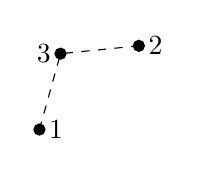
\begin{tikzpicture}
\draw[dashed]  (0,0)-- (0.2674988286, 0.9635581854)--(1.262502994, 1.063391602);
\filldraw[black] (0,0) circle (2pt) node[anchor=west]{1};
\filldraw[black] (0.2674988286, 0.9635581854) circle (2pt) node[anchor=east]{3};
\filldraw[black] (1.262502994, 1.063391602) circle (2pt) node[anchor=west]{2};
\end{tikzpicture}
    \end{subfigure}
    \begin{subfigure}[b]{.2\textwidth}
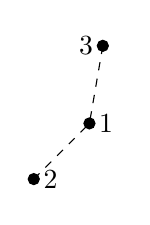
\begin{tikzpicture}
\draw[dashed]  (0.1699671429, 0.9854497300)--(0,0)--(-0.7071067805, -0.7071067810);
\filldraw[black] (0,0) circle (2pt) node[anchor=west]{1};
\filldraw[black] (0.1699671429, 0.9854497300) circle (2pt) node[anchor=east]{3};
\filldraw[black] (-0.7071067805, -0.7071067810) circle (2pt) node[anchor=west]{2};
\end{tikzpicture}
    \end{subfigure}
    \begin{subfigure}[b]{.2\textwidth}
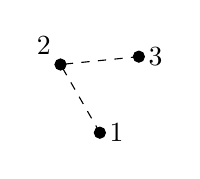
\begin{tikzpicture}
\draw[dashed]  (0,0)-- (-0.5000000005, 0.8660254035)--(0.4950041648, 0.9658588202);
\filldraw[black] (0,0) circle (2pt) node[anchor=west]{1};
\filldraw[black] (-0.5000000005, 0.8660254035) circle (2pt) node[anchor=south east]{2};
\filldraw[black] (0.4950041648, 0.9658588202) circle (2pt) node[anchor=west]{3};
\end{tikzpicture}
    \end{subfigure}
     \begin{subfigure}[b]{.2\textwidth}
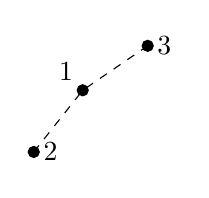
\begin{tikzpicture}
\draw[dashed]  (0,0)-- (0.6216099683, 0.7833269096)--(1.446945583, 1.347969383);
\filldraw[black] (0,0) circle (2pt) node[anchor=west]{2};
\filldraw[black] (0.6216099683, 0.7833269096) circle (2pt) node[anchor=south east]{1};
\filldraw[black] (1.446945583, 1.347969383) circle (2pt) node[anchor=west]{3};
\end{tikzpicture}
    \end{subfigure}
    \caption{Some points in configuration space.}
    \label{fig:confex}
\end{figure}

We then chose the corresponding density estimator $f(x)$ with values of 
$h=.25$ in the $L^2$ metric, which does not represent a uniform measure on the underlying space in any sense. We computed $\denswit(f,\dataset_{\geq .006},.4)$ up to the 3-simplices, and obtained a 3-dimensional filtered complex with sizes (271,1264,1558,631). The persistent homology groups are shown in Figure \ref{fig:config}. The bars which extend indefinitely correspond to the desired betti numbers of $\conf_3(\mathbb{R}^2)$ given by $(\betti_0,\betti_1,\betti_2)=(1,3,2)$. We also see that in the medium density range, we have a value of $\betti_0=2$ and $\betti_1=2$, whose bars are too long to be due to noise. This is due to the fact that the triples which nearly form an equilateral triangle tend to be denser that triples which are colinear. As a result, we obtain two disconnected loops in the medium density range, corresponding to the two rotationally inequivalent permutations of the labels, when the points lie on an equilateral triangle.

\begin{figure}
    \centering
    \includegraphics[scale=.35]{figures/config/config1.png}
    \caption{Persistent homology groups of the Configuration space data set.}
    \label{fig:config}
\end{figure}


\end{example}

\subsection{Local patches from the MNIST data set}

\label{sec:patches}

In \cite{carlsson2008klein},
the authors studied the topology of a certain space of  local $3\times 3$ high intensity patches of the van Hateren data set of natural images, which was investigated earlier by Lee, Mumford, and Pederson \cite{hateren_schaaf_1998,mumford2003nonlinear}. They gave quantitative evidence using the witness complex that those patches lie along a two-dimensional locus parametrized by the Klein bottle. 


We illustrate our complex on a parallel construction of high intensity local patches in the MNIST data set of $28 \times 28$ images of hand-drawn digits \cite{deng2012mnist}. Because digits tend to have lines in the middle of blank space, but rarely the reverse, we expect those patches to lie in a sublocus of the Klein bottle homeomorphic to the M\"{o}bius strip. Some points in the MNIST data set and a parametrization of this M\"{o}bius strip are shown in the first two rows of Figure \ref{fig:mnist}. 
The circle that traces around the boundary of the M\"{o}bius strip through the top and bottom row is called the primary circle, and it usually contains points of higher density than those in the middle row.
The circle consisting of the middle row is called the secondary circle, and it is more difficult to detect. We will see that the density based complex exhibits 
descriptive visual models of both primary and secondary circle features, with clear differences between different digits.




To form a parametrization of image patches, we considered an inner product on the $l^2$-dimensional vector space $\mat(l,l)$ of $l\times l$ image patches, given by
\begin{equation}
    \label{eq:hermsp}
(A,B)=\frac{1}{2^{2(l-1)}}\sum_{i=1}^l \sum_{j=1}^l
\binom{l-1}{i-1} \binom{l-1}{j-1}
A_{i,j} B_{i,j}
\end{equation}
We then consider an orthonormal basis 
given by $H_{a,b}^l=H^l_a \otimes H^l_b$, where the $H_a \in \mathbb{R}^l$ are a discrete form of the Hermite polynomials,
given by applying the Gram-Schmidt algorithm to the vectors of polynomial functions $V^a=(i^a)_{i=1}^l$, using the one-dimensional form of \eqref{eq:hermsp}.
For several reasons, we find the inner product to be more robust than the usual dot product, which would lead to products of Legendre polynomials.
The bottom row of Figure \ref{fig:mnist} shows an example of two such vectors, and the result of projecting an image patch  onto the span of the 6 Hermite polynomials up to quadratic order for $l=7$.


We then constructed a data set as follows. For 50 instances each digit, we sampled all $l\times l$ patches for various choice of $l$, and projected those patches onto $\spn(H^l_{1,0},H^l_{0,1},H^l_{2,0},H^l_{1,1},H^l_{0,2})$, the span of nonconstant terms up to quadratic order, to obtain a data set of size $50\cdot 28\cdot 28=39200$ in $\mathbb{R}^5$ (assuming that patches are extended by zero outside the domain of the image). We then chose only those images whose norm is above a fixed number of $r=.3$, resulting in a subset of roughly $10\%$ of the original size. This is a version of the choice of ``high intensity patches'' 
from \cite{carlsson2008klein}. We then normalized the resulting points to arrive at a data set $\dataset(k)\subset S^4$ of size 3000-5000 for each digit $k\in \{0,...,9\}$.

We show the results of $\denswit(f,\domain,s)$ using the values of $l=11$, $h=.16$, $\domain=\dataset(k)_{\geq \mindens}$, $s=.5$, with varying choices of $\mindens$ in the top row of Figure \ref{fig:patches1}. We see that primary circle features are dominant, corresponding to the dense regions around the periphery, with secondary circle features connecting them. The coordinate system is the one spanned by $H^{11}_{1,0},H^{11}_{0,1}$. In order to highlight the secondary circle features, we produced a variant on the above data set, in which high intensity is determined only by the norm of the quadratic terms, and in which we normalize by that value. This has the effect of dimensionally reducing just the second degree terms, thereby accentuating the secondary circle. We then mapped the resulting complexes into low dimension using a similar parametrization of the Klein bottle to the one given in \cite{carlsson2008klein}. In the case of the digit $0$, we see a very clear M\"{o}bius strip. In the case of the digit 2, we lowered the density threshold, revealing a primary circle feature encircling the second order ones.


\begin{figure}
    \centering
        \begin{subfigure}[b]{.24\textwidth}    \includegraphics[scale=.27]{figures/patches/patch1.png}
    \end{subfigure}
        \begin{subfigure}[b]{.24\textwidth}    \includegraphics[scale=.27]{figures/patches/patch7.png}
    \end{subfigure}        
        \begin{subfigure}[b]{.24\textwidth}    \includegraphics[scale=.27]{figures/patches/patch0.png}
    \end{subfigure}     
        \begin{subfigure}[b]{.24\textwidth}    \includegraphics[scale=.27]{figures/patches/patch2.png}
    \end{subfigure}

\hspace{0.3\textwidth}

    
   \centering
    \begin{subfigure}[b]{.1\textwidth}
    \includegraphics[scale=1.27]{figures/klein/klein20.png}
    \end{subfigure}
        \begin{subfigure}[b]{.1\textwidth}
    \includegraphics[scale=1.27]{figures/klein/klein21.png}
    \end{subfigure}
        \begin{subfigure}[b]{.1\textwidth}
    \includegraphics[scale=1.27]{figures/klein/klein22.png}
    \end{subfigure}
        \begin{subfigure}[b]{.1\textwidth}
    \includegraphics[scale=1.27]{figures/klein/klein23.png}
    \end{subfigure}
        \begin{subfigure}[b]{.1\textwidth}
    \includegraphics[scale=1.27]{figures/klein/klein24.png}
    \end{subfigure}
           \begin{subfigure}[b]{.1\textwidth}
           \includegraphics[scale=1.27]
    {figures/klein/klein25.png}
    \end{subfigure}
        \begin{subfigure}[b]{.1\textwidth}
    \includegraphics[scale=1.27]{figures/klein/klein26.png}
    \end{subfigure}
        \begin{subfigure}[b]{.1\textwidth}
    \includegraphics[scale=1.27]{figures/klein/klein27.png}
    \end{subfigure}
        \begin{subfigure}[b]{.1\textwidth}
    \includegraphics[scale=1.27]{figures/klein/klein28.png}
    \end{subfigure}



    \centering
    \begin{subfigure}[b]{.1\textwidth}
    \includegraphics[scale=1.27]{figures/klein/klein30.png}
    \end{subfigure}
        \begin{subfigure}[b]{.1\textwidth}
    \includegraphics[scale=1.27]{figures/klein/klein31.png}
    \end{subfigure}
        \begin{subfigure}[b]{.1\textwidth}
    \includegraphics[scale=1.27]{figures/klein/klein32.png}
    \end{subfigure}
        \begin{subfigure}[b]{.1\textwidth}
    \includegraphics[scale=1.27]{figures/klein/klein33.png}
    \end{subfigure}
        \begin{subfigure}[b]{.1\textwidth}
    \includegraphics[scale=1.27]{figures/klein/klein34.png}
    \end{subfigure}
           \begin{subfigure}[b]{.1\textwidth}
           \includegraphics[scale=1.27]
    {figures/klein/klein35.png}
    \end{subfigure}
        \begin{subfigure}[b]{.1\textwidth}
    \includegraphics[scale=1.27]{figures/klein/klein36.png}
    \end{subfigure}
        \begin{subfigure}[b]{.1\textwidth}
    \includegraphics[scale=1.27]{figures/klein/klein37.png}
    \end{subfigure}
        \begin{subfigure}[b]{.1\textwidth}
    \includegraphics[scale=1.27]{figures/klein/klein38.png}
    \end{subfigure}





    \centering
    \begin{subfigure}[b]{.1\textwidth}
    \includegraphics[scale=1.27]{figures/klein/klein40.png}
    \end{subfigure}
        \begin{subfigure}[b]{.1\textwidth}
    \includegraphics[scale=1.27]{figures/klein/klein41.png}
    \end{subfigure}
        \begin{subfigure}[b]{.1\textwidth}
    \includegraphics[scale=1.27]{figures/klein/klein42.png}
    \end{subfigure}
        \begin{subfigure}[b]{.1\textwidth}
    \includegraphics[scale=1.27]{figures/klein/klein43.png}
    \end{subfigure}
        \begin{subfigure}[b]{.1\textwidth}
    \includegraphics[scale=1.27]{figures/klein/klein44.png}
    \end{subfigure}
           \begin{subfigure}[b]{.1\textwidth}
           \includegraphics[scale=1.27]
    {figures/klein/klein45.png}
    \end{subfigure}
        \begin{subfigure}[b]{.1\textwidth}
    \includegraphics[scale=1.27]{figures/klein/klein46.png}
    \end{subfigure}
        \begin{subfigure}[b]{.1\textwidth}
    \includegraphics[scale=1.27]{figures/klein/klein47.png}
    \end{subfigure}
        \begin{subfigure}[b]{.1\textwidth}
    \includegraphics[scale=1.27]{figures/klein/klein48.png}
    \end{subfigure}



    \centering
    \begin{subfigure}[b]{.1\textwidth}
    \includegraphics[scale=1.27]{figures/klein/klein50.png}
    \end{subfigure}
        \begin{subfigure}[b]{.1\textwidth}
    \includegraphics[scale=1.27]{figures/klein/klein51.png}
    \end{subfigure}
        \begin{subfigure}[b]{.1\textwidth}
    \includegraphics[scale=1.27]{figures/klein/klein52.png}
    \end{subfigure}
        \begin{subfigure}[b]{.1\textwidth}
    \includegraphics[scale=1.27]{figures/klein/klein53.png}
    \end{subfigure}
        \begin{subfigure}[b]{.1\textwidth}
    \includegraphics[scale=1.27]{figures/klein/klein54.png}
    \end{subfigure}
           \begin{subfigure}[b]{.1\textwidth}
           \includegraphics[scale=1.27]
    {figures/klein/klein55.png}
    \end{subfigure}
        \begin{subfigure}[b]{.1\textwidth}
    \includegraphics[scale=1.27]{figures/klein/klein56.png}
    \end{subfigure}
        \begin{subfigure}[b]{.1\textwidth}
    \includegraphics[scale=1.27]{figures/klein/klein57.png}
    \end{subfigure}
        \begin{subfigure}[b]{.1\textwidth}
    \includegraphics[scale=1.27]{figures/klein/klein58.png}
    \end{subfigure}



    \centering
    \begin{subfigure}[b]{.1\textwidth}
    \includegraphics[scale=1.27]{figures/klein/klein60.png}
    \end{subfigure}
        \begin{subfigure}[b]{.1\textwidth}
    \includegraphics[scale=1.27]{figures/klein/klein61.png}
    \end{subfigure}
        \begin{subfigure}[b]{.1\textwidth}
    \includegraphics[scale=1.27]{figures/klein/klein62.png}
    \end{subfigure}
        \begin{subfigure}[b]{.1\textwidth}
    \includegraphics[scale=1.27]{figures/klein/klein63.png}
    \end{subfigure}
        \begin{subfigure}[b]{.1\textwidth}
    \includegraphics[scale=1.27]{figures/klein/klein64.png}
    \end{subfigure}
           \begin{subfigure}[b]{.1\textwidth}
           \includegraphics[scale=1.27]
    {figures/klein/klein65.png}
    \end{subfigure}
        \begin{subfigure}[b]{.1\textwidth}
    \includegraphics[scale=1.27]{figures/klein/klein66.png}
    \end{subfigure}
        \begin{subfigure}[b]{.1\textwidth}
    \includegraphics[scale=1.27]{figures/klein/klein67.png}
    \end{subfigure}
        \begin{subfigure}[b]{.1\textwidth}
    \includegraphics[scale=1.27]{figures/klein/klein68.png}
    \end{subfigure}




    
   


\hspace{0.3\textwidth}

    \centering
        \begin{subfigure}[b]{.24\textwidth}    \includegraphics[scale=1.05]{figures/patches/patch2a.png}
    \end{subfigure}
        \begin{subfigure}[b]{.24\textwidth}    \includegraphics[scale=1.05]{figures/patches/patch2b.png}
    \end{subfigure}        
        \begin{subfigure}[b]{.24\textwidth}    \includegraphics[scale=1.05]{figures/patches/patch2c.png}
    \end{subfigure}
    \begin{subfigure}[b]{.24\textwidth}    \includegraphics[scale=1.05]{figures/patches/patch2d.png}
    \end{subfigure}
    
    \caption{Top row: some elements from the MNIST data set of $28\times 28$ grayscale images of hand drawn digits. Middle row: a M\"{o}bius strip in the space of image patches. Bottom row: on the left are two instances of the Hermite polynomials
    $H^7_{0,1}$ and $H^7_{1,1}$. In the second from the right, a typical $7\times 7$ patch from the data set, and its projection onto the span of the Hermite polynomials up to quadratic order on the far right.}
    \label{fig:mnist}
\end{figure}






\begin{figure}
    \centering
\begin{subfigure}[b]{.24\textwidth}
    \includegraphics[scale=.5]{figures/patches/patches1.pdf}
    \caption{Digit 1}
\end{subfigure}
\begin{subfigure}[b]{.24\textwidth}  
      \includegraphics[scale=.5]{figures/patches/patches7.pdf}
          \caption{Digit 7}
\end{subfigure}
\begin{subfigure}[b]{.24\textwidth}
    \includegraphics[scale=.5]{figures/patches/patches0.pdf}
          \caption{Digit 0}
\end{subfigure}
\begin{subfigure}[b]{.24\textwidth}
    \includegraphics[scale=.5]{figures/patches/patches2.pdf}
          \caption{Digit 2}
\end{subfigure}

    \centering
\begin{subfigure}[b]{.24\textwidth}
    \includegraphics[scale=.45]{figures/patches/mobius1.pdf}
    \caption{Digit 1}
\end{subfigure}
\begin{subfigure}[b]{.24\textwidth}  
      \includegraphics[scale=.45]{figures/patches/mobius7.pdf}
          \caption{Digit 7}
\end{subfigure}
\begin{subfigure}[b]{.24\textwidth}
    \includegraphics[scale=.45]{figures/patches/mobius0.pdf}
          \caption{Digit 0}
\end{subfigure}
\begin{subfigure}[b]{.24\textwidth}
    \includegraphics[scale=.45]{figures/patches/mobius2.pdf}
          \caption{Digit 2}
\end{subfigure}
    \caption{Top row: The complex 
    $\denswit(f,\domain,s)$ for the digits $\{1,7,0,2\}$. All have the same parameters $h=.16$, $s=.5$, $r=.3$, and varying choices of $\mindens$.
Bottom row: a similar construction but defining intensity using only the second order features.}
    \label{fig:patches1}
\end{figure}


\subsection{The Ising model on a graph}

\label{sec:ising}

In our final example, we consider density estimation on a simulated data set consisting of trials of the Ising model \cite{ising1925ferromagetism} on a graph with $m$ vertices, thought of as a collection of real-valued vectors in $\R^m$.
In order to obtain a viable density estimator on this data set, we use the Laplacian operator associated to the graph, which has the effect of replacing each trial by something resembling a continuous function.


Let $G=(V,E)$ be an $m\times m$ graph such as the ones shown in Figure \ref{fig:isinggraphs}, represented by a symmetric adjacency matrix $J$, diagonal entries being zero. For every discrete vector 
of ``spins'' $\sigma \in \{1,-1\}^m$, we have the Hamiltonian energy
\begin
{equation}
\label{eq:isingham}
    H_G(\sigma)=-\sum_{i,j}
J_{i,j} \sigma_i \sigma_j=
H_{\min}+2|\{(i,j)\in E: \sigma_i\neq \sigma_j\}|.
\end{equation}
Those points $(i,j)\in E$ for which $\sigma_i\neq \sigma_j$ are called transitions.
For each choice of $\beta>0$, called the temperature parameter, one seeks to sample from the
Boltzmann distribution on $\{1,-1\}^m$
given by
\begin{equation}
    \label{eq:boltzmann}
P_{\beta}(\sigma)=\frac{1}{Z_{\beta}}
e^{-\beta H(\sigma)},\quad
Z_\beta = \sum_{\sigma} e^{-\beta H(\sigma)}
\end{equation}
which is done using the single-flip Metropolis algorithm. 

\begin{figure}[t]
\centering
 \begin{subfigure}[b]{.3\textwidth}
\begin{tikzpicture}[scale=.25]
\draw[color=white] (-6.5,-6) rectangle (6.5,6);


\draw[color=black!100,thick] (-4.833333,0)--(-4.500000,0);
\draw[color=black!100,thick] (-4.500000,0)--(-4.166667,0);
\draw[color=black!100,thick] (-4.166667,0)--(-3.833333,0);
\draw[color=black!100,thick] (-3.833333,0)--(-3.500000,0);
\draw[color=black!100,thick] (-3.500000,0)--(-3.166667,0);
\draw[color=black!100,thick] (-3.166667,0)--(-2.833333,0);
\draw[color=black!100,thick] (-2.833333,0)--(-2.500000,0);
\draw[color=black!100,thick] (-2.500000,0)--(-2.166667,0);
\draw[color=black!100,thick] (-2.166667,0)--(-1.833333,0);
\draw[color=black!100,thick] (-1.833333,0)--(-1.500000,0);
\draw[color=black!100,thick] (-1.500000,0)--(-1.166667,0);
\draw[color=black!100,thick] (-1.166667,0)--(-0.833333,0);
\draw[color=black!100,thick] (-0.833333,0)--(-0.500000,0);
\draw[color=black!100,thick] (-0.500000,0)--(-0.166667,0);
\draw[color=black!100,thick] (-0.166667,0)--(0.166667,0);
\draw[color=black!100,thick] (0.166667,0)--(0.500000,0);
\draw[color=black!100,thick] (0.500000,0)--(0.833333,0.0);
\draw[color=black!100,thick] (0.833333,0)--(1.166667,0);
\draw[color=black!100,thick] (1.166667,0)--(1.500000,0);
\draw[color=black!100,thick] (1.500000,0)--(1.833333,0);
\draw[color=black!100,thick] (1.833333,0)--(2.166667,0);
\draw[color=black!100,thick] (2.166667,0)--(2.500000,0);
\draw[color=black!100,thick] (2.500000,0)--(2.833333,0);
\draw[color=black!100,thick] (2.833333,0)--(3.166667,0);
\draw[color=black!100,thick] (3.166667,0)--(3.500000,0);
\draw[color=black!100,thick] (3.500000,0)--(3.833333,0);
\draw[color=black!100,thick] (3.833333,0)--(4.166667,0);
\draw[color=black!100,thick] (4.166667,0)--(4.500000,0);
\draw[color=black!100,thick] (4.5,0)--(5.166666,0);


\draw[color=black!100,fill=black!100,thick] (-4.833333,0) circle (4.0pt);

\draw[color=black!100,fill=black!100,thick] (-3.833333,0) circle (4.0pt);

\draw[color=black!100,fill=black!100,thick] (-2.833333,0) circle (4.0pt);

\draw[color=black!100,fill=black!100,thick] (-1.833333,0) circle (4.0pt);

\draw[color=black!100,fill=black!100,thick] (-0.833333,0) circle (4.0pt);

\draw[color=black!100,fill=black!100,thick] (0.166667,0) circle (4.0pt);

\draw[color=black!100,fill=black!100,thick] (1.166667,0) circle (4.0pt);

\draw[color=black!100,fill=black!100,thick] (2.166667,0) circle (4.0pt);

\draw[color=black!100,fill=black!100,thick] (3.166667,0) circle (4.0pt);

\draw[color=black!100,fill=black!100,thick] (4.166667,0) circle (4.0pt);

\draw[color=black!100,fill=black!100,thick] (5.1666667,0) circle (4.0pt);


\end{tikzpicture}
\end{subfigure}
\begin{subfigure}[b]{.3\textwidth}
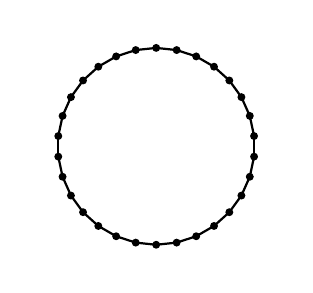
\begin{tikzpicture}[scale=.25]
\draw[color=white] (-6.5,-6) rectangle (6.5,6);


\draw[color=black!100,thick] (4.972609,0.522642)--(4.755283,1.545085);
\draw[color=black!100,thick] (4.755283,1.545085)--(4.330127,2.500000);
\draw[color=black!100,thick] (4.330127,2.500000)--(3.715724,3.345653);
\draw[color=black!100,thick] (3.715724,3.345653)--(2.938926,4.045085);
\draw[color=black!100,thick] (2.938926,4.045085)--(2.033683,4.567727);
\draw[color=black!100,thick] (2.033683,4.567727)--(1.039558,4.890738);
\draw[color=black!100,thick] (1.039558,4.890738)--(-0.000000,5.000000);
\draw[color=black!100,thick] (-0.000000,5.000000)--(-1.039558,4.890738);
\draw[color=black!100,thick] (-1.039558,4.890738)--(-2.033683,4.567727);
\draw[color=black!100,thick] (-2.033683,4.567727)--(-2.938926,4.045085);
\draw[color=black!100,thick] (-2.938926,4.045085)--(-3.715724,3.345653);
\draw[color=black!100,thick] (-3.715724,3.345653)--(-4.330127,2.500000);
\draw[color=black!100,thick] (-4.330127,2.500000)--(-4.755283,1.545085);
\draw[color=black!100,thick] (-4.755283,1.545085)--(-4.972609,0.522642);
\draw[color=black!100,thick] (-4.972609,0.522642)--(-4.972609,-0.522642);
\draw[color=black!100,thick] (-4.972609,-0.522642)--(-4.755283,-1.545085);
\draw[color=black!100,thick] (-4.755283,-1.545085)--(-4.330127,-2.500000);
\draw[color=black!100,thick] (-4.330127,-2.500000)--(-3.715724,-3.345653);
\draw[color=black!100,thick] (-3.715724,-3.345653)--(-2.938926,-4.045085);
\draw[color=black!100,thick] (-2.938926,-4.045085)--(-2.033683,-4.567727);
\draw[color=black!100,thick] (-2.033683,-4.567727)--(-1.039558,-4.890738);
\draw[color=black!100,thick] (-1.039558,-4.890738)--(0.000000,-5.000000);
\draw[color=black!100,thick] (0.000000,-5.000000)--(1.039558,-4.890738);
\draw[color=black!100,thick] (1.039558,-4.890738)--(2.033683,-4.567727);
\draw[color=black!100,thick] (2.033683,-4.567727)--(2.938926,-4.045085);
\draw[color=black!100,thick] (2.938926,-4.045085)--(3.715724,-3.345653);
\draw[color=black!100,thick] (3.715724,-3.345653)--(4.330127,-2.500000);
\draw[color=black!100,thick] (4.330127,-2.500000)--(4.755283,-1.545085);
\draw[color=black!100,thick] (4.755283,-1.545085)--(4.972609,-0.522642);
\draw[color=black!100,thick] (4.972609,-0.522642)--(4.972609,0.522642);


\draw[color=black!100,fill=black!100,thick] (4.972609,0.522642) circle (4.0pt);
\draw[color=black!100,fill=black!100,thick] (4.755283,1.545085) circle (4.0pt);
\draw[color=black!100,fill=black!100,thick] (4.330127,2.500000) circle (4.0pt);
\draw[color=black!100,fill=black!100,thick] (3.715724,3.345653) circle (4.0pt);
\draw[color=black!100,fill=black!100,thick] (2.938926,4.045085) circle (4.0pt);
\draw[color=black!100,fill=black!100,thick] (2.033683,4.567727) circle (4.0pt);
\draw[color=black!100,fill=black!100,thick] (1.039558,4.890738) circle (4.0pt);
\draw[color=black!100,fill=black!100,thick] (-0.000000,5.000000) circle (4.0pt);
\draw[color=black!100,fill=black!100,thick] (-1.039558,4.890738) circle (4.0pt);
\draw[color=black!100,fill=black!100,thick] (-2.033683,4.567727) circle (4.0pt);
\draw[color=black!100,fill=black!100,thick] (-2.938926,4.045085) circle (4.0pt);
\draw[color=black!100,fill=black!100,thick] (-3.715724,3.345653) circle (4.0pt);
\draw[color=black!100,fill=black!100,thick] (-4.330127,2.500000) circle (4.0pt);
\draw[color=black!100,fill=black!100,thick] (-4.755283,1.545085) circle (4.0pt);
\draw[color=black!100,fill=black!100,thick] (-4.972609,0.522642) circle (4.0pt);
\draw[color=black!100,fill=black!100,thick] (-4.972609,-0.522642) circle (4.0pt);
\draw[color=black!100,fill=black!100,thick] (-4.755283,-1.545085) circle (4.0pt);
\draw[color=black!100,fill=black!100,thick] (-4.330127,-2.500000) circle (4.0pt);
\draw[color=black!100,fill=black!100,thick] (-3.715724,-3.345653) circle (4.0pt);
\draw[color=black!100,fill=black!100,thick] (-2.938926,-4.045085) circle (4.0pt);
\draw[color=black!100,fill=black!100,thick] (-2.033683,-4.567727) circle (4.0pt);
\draw[color=black!100,fill=black!100,thick] (-1.039558,-4.890738) circle (4.0pt);
\draw[color=black!100,fill=black!100,thick] (0.000000,-5.000000) circle (4.0pt);
\draw[color=black!100,fill=black!100,thick] (1.039558,-4.890738) circle (4.0pt);
\draw[color=black!100,fill=black!100,thick] (2.033683,-4.567727) circle (4.0pt);
\draw[color=black!100,fill=black!100,thick] (2.938926,-4.045085) circle (4.0pt);
\draw[color=black!100,fill=black!100,thick] (3.715724,-3.345653) circle (4.0pt);
\draw[color=black!100,fill=black!100,thick] (4.330127,-2.500000) circle (4.0pt);
\draw[color=black!100,fill=black!100,thick] (4.755283,-1.545085) circle (4.0pt);
\draw[color=black!100,fill=black!100,thick] (4.972609,-0.522642) circle (4.0pt);
\end{tikzpicture}
\end{subfigure}
\begin{subfigure}[b]{.3\textwidth}
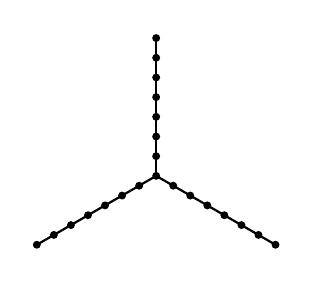
\begin{tikzpicture}[scale=.25]
\draw[color=white] (-6.5,-4.5) rectangle (6.5,7.5);

\draw[color=black!100,thick] (0.000000,0.000000)--(0.000000,0.500000);
\draw[color=black!100,thick] (0.000000,0.500000)--(0.000000,1.000000);
\draw[color=black!100,thick] (0.000000,1.000000)--(0.000000,1.500000);
\draw[color=black!100,thick] (0.000000,1.500000)--(0.000000,2.000000);
\draw[color=black!100,thick] (0.000000,2.000000)--(0.000000,2.500000);
\draw[color=black!100,thick] (0.000000,2.500000)--(0.000000,3.000000);
\draw[color=black!100,thick] (0.000000,3.000000)--(0.000000,3.500000);
\draw[color=black!100,thick] (0.000000,3.500000)--(0.000000,4.000000);
\draw[color=black!100,thick] (0.000000,4.000000)--(0.000000,4.500000);
\draw[color=black!100,thick] (0.000000,4.500000)--(0.000000,5.000000);
\draw[color=black!100,thick] (0.000000,5.000000)--(0.000000,5.500000);
\draw[color=black!100,thick] (0.000000,5.500000)--(0.000000,6.000000);
\draw[color=black!100,thick] (0.000000,6.000000)--(0.000000,6.500000);
\draw[color=black!100,thick] (0.000000,6.500000)--(0.000000,7.000000);

\draw[color=black!100,thick] (0.000000,0.000000)--(-0.433013,-0.250000);
\draw[color=black!100,thick] (-0.433013,-0.250000)--(-0.866025,-0.500000);
\draw[color=black!100,thick] (-0.866025,-0.500000)--(-1.299038,-0.750000);
\draw[color=black!100,thick] (-1.299038,-0.750000)--(-1.732051,-1.000000);
\draw[color=black!100,thick] (-1.732051,-1.000000)--(-2.165064,-1.250000);
\draw[color=black!100,thick] (-2.165064,-1.250000)--(-2.598076,-1.500000);
\draw[color=black!100,thick] (-2.598076,-1.500000)--(-3.031089,-1.750000);
\draw[color=black!100,thick] (-3.031089,-1.750000)--(-3.464102,-2.000000);
\draw[color=black!100,thick] (-3.464102,-2.000000)--(-3.897114,-2.250000);
\draw[color=black!100,thick] (-3.897114,-2.250000)--(-4.330127,-2.500000);
\draw[color=black!100,thick] (-4.330127,-2.500000)--(-4.763140,-2.750000);
\draw[color=black!100,thick] (-4.763140,-2.750000)--(-5.196152,-3.000000);
\draw[color=black!100,thick] (-5.196152,-3.000000)--(-5.629165,-3.250000);
\draw[color=black!100,thick] (-5.629165,-3.250000)--(-6.062178,-3.500000);


\draw[color=black!100,thick] (0.000000,0.000000)--(0.433013,-0.250000);
\draw[color=black!100,thick] (0.433013,-0.250000)--(0.866025,-0.500000);
\draw[color=black!100,thick] (0.866025,-0.500000)--(1.299038,-0.750000);
\draw[color=black!100,thick] (1.299038,-0.750000)--(1.732051,-1.000000);
\draw[color=black!100,thick] (1.732051,-1.000000)--(2.165064,-1.250000);
\draw[color=black!100,thick] (2.165064,-1.250000)--(2.598076,-1.500000);
\draw[color=black!100,thick] (2.598076,-1.500000)--(3.031089,-1.750000);
\draw[color=black!100,thick] (3.031089,-1.750000)--(3.464102,-2.000000);
\draw[color=black!100,thick] (3.464102,-2.000000)--(3.897114,-2.250000);
\draw[color=black!100,thick] (3.897114,-2.250000)--(4.330127,-2.500000);
\draw[color=black!100,thick] (4.330127,-2.500000)--(4.763140,-2.750000);
\draw[color=black!100,thick] (4.763140,-2.750000)--(5.196152,-3.000000);
\draw[color=black!100,thick] (5.196152,-3.000000)--(5.629165,-3.250000);
\draw[color=black!100,thick] (5.629165,-3.250000)--(6.062178,-3.500000);


\draw[color=black!100,fill=black!100,thick] (0.000000,1.000000) circle (4.0pt);
\draw[color=black!100,fill=black!100,thick] (0.000000,2.000000) circle (4.0pt);
\draw[color=black!100,fill=black!100,thick] (0.000000,3.000000) circle (4.0pt);
\draw[color=black!100,fill=black!100,thick] (0.000000,4.000000) circle (4.0pt);
\draw[color=black!100,fill=black!100,thick] (0.000000,5.000000) circle (4.0pt);
\draw[color=black!100,fill=black!100,thick] (0.000000,6.000000) circle (4.0pt);
\draw[color=black!100,fill=black!100,thick] (0.000000,7.000000) circle (4.0pt);


\draw[color=black!100,fill=black!100,thick] (0.866025,-0.500000) circle (4.0pt);
\draw[color=black!100,fill=black!100,thick] (1.732051,-1.000000) circle (4.0pt);
\draw[color=black!100,fill=black!100,thick] (2.598076,-1.500000) circle (4.0pt);
\draw[color=black!100,fill=black!100,thick] (3.464102,-2.000000) circle (4.0pt);
\draw[color=black!100,fill=black!100,thick] (4.330127,-2.500000) circle (4.0pt);
\draw[color=black!100,fill=black!100,thick] (5.196152,-3.000000) circle (4.0pt);
\draw[color=black!100,fill=black!100,thick] (6.062178,-3.500000) circle (4.0pt);


\draw[color=black!100,fill=black!100,thick] (-0.866025,-0.500000) circle (4.0pt);
\draw[color=black!100,fill=black!100,thick] (-1.732051,-1.000000) circle (4.0pt);
\draw[color=black!100,fill=black!100,thick] (-2.598076,-1.500000) circle (4.0pt);
\draw[color=black!100,fill=black!100,thick] (-3.464102,-2.000000) circle (4.0pt);
\draw[color=black!100,fill=black!100,thick] (-4.330127,-2.500000) circle (4.0pt);
\draw[color=black!100,fill=black!100,thick] (-5.196152,-3.000000) circle (4.0pt);
\draw[color=black!100,fill=black!100,thick] (-6.062178,-3.500000) circle (4.0pt);

\draw[color=black!100,fill=black!100,thick] (0.000000,0.000000) circle (4.0pt);

\end{tikzpicture}
\end{subfigure}
\caption{Top row: three different graphs $G$ used to simulate the Ising model, denoted $\isingint(11)$, $\isingcirc(30)$, $\isingflares(22)$. The index corresponds to the number of vertices.}
\label{fig:isinggraphs}
 \end{figure}

A collection of $N$ trials can be interpreted as a data set
\[\mathcal{D}(G,\beta)=
\{\sigma^1,...,\sigma^N\} \subset \mathbb{R}^m,\] 
by viewing the
spin states $\sigma$ as real vectors in $\mathbb{R}^m$.
We generated $\mathcal{D}(G,\beta)$ for the three different types of
graph $G$ shown in Figure \ref{fig:isinggraphs}, but with different numbers of vertices. Specifically, we took an interval consisting of 30 sites, a circle with 30 sites, and a graph with three flares of length 14 each coming from the center, for a total of 43 vertices. For every one we chose $\beta=1.5$, and $N=20000$. 
In the case of the interval, the distribution of the energy values is given by
\[(a_k)= (4907,7035, 4942, 2193, 709, 167, 41, 6, 0,...)\]
where $a_k$ is the number of states $\sigma\in \dataset$ with $k$ transitions. For instance, 
we would have 4907 instances in which all spins are the same, and 6 instances in which there are 7 transitions. These numbers are consistent with the predicted values, which by a simple combinatorial argument are proportional to
\[a_k \sim \binom{m-1}{k}/2^{m-1} e^{-2\beta k}\]
for the given parameters.
 \begin{figure}
 \centering
\begin{subfigure}[b]{.35\textwidth}
    \includegraphics[scale=1.0]{figures/ising/laplacian1a.pdf}
\end{subfigure}
\begin{subfigure}[b]{.35\textwidth}
        \includegraphics[scale=1.0]{figures/ising/laplacian2a.pdf}
\end{subfigure}
    \caption{On the left: a typical data point
    in $\dataset(G,\beta)$ with three transitions
    for $(G,\beta)=(\isingflares(43),1.5)$.
    The spins $\pm 1$ are represented by black and white. On the right: the same point after diffusion, i.e. right multiplication by
    $\exp(-tL^t)$ for $t=10$.}
    \label{fig:laplacian}
\end{figure}

Applying density estimation to these spaces directly would be subject to the curse of dimensionality, and would not produce useful results. Instead of a dimensional reduction, we will consider a blended form of the data set using the left-normalized Laplacian operator 
$I-D^{-1}A$. Here $A$ is the adjacency matrix of $G$, normalized so that the diagonal entry $A_{i,i}$ is the degree of $v_i$, and $D$ is the row-sum of $A$. There are several reasons for this choice of diagonal in $A$, for instance a troublesome dependence of the eigenvalues of $L^{t}$ on the parity of $m$ when the diagonal entries are zero. 
In the case of the interval with $30$ vertices, the first few values of these eigenvalues are
\[\Lambda=(1.000, .997, .988, .974, .954, .928, .898, .863, .824, .781,...).\]
We then make the replacement $\dataset(G,\beta)\mapsto \dataset(G,\beta)\exp(-tL^{t})$ with the value of $t=10$, viewing the data set as an $N\times m$ matrix,
to produce a continuous form of each data point as shown in Figure \ref{fig:laplacian}.

We then chose the density estimator $f(x)$ with scale parameter $h=2.0$, and computed
$Y=\denswit(f,\dataset(\beta,J)_{\geq .001},.4)$
for each graph $G$ up to the 3-simplices. In the case of the 
$G=\isingint(30)$, we obtain a filtered complex with sizes $(|Y_0|,|Y_1|,|Y_2|,|Y_3|)=(210,2213,6500,8570)$.
The persistent homology groups, shown in Figure \ref{fig:isingjava}, show the betti numbers of low energy states, which are the ones of higher density. For instance, the $\betti_0$ barcodes show two connected components at high density, corresponding to the two states in which all spins are the same.

\begin{figure}
    \centering\includegraphics[scale=.35]{figures/ising/ising1.png}
    \caption{Persistent homology groups of $\denswit(f,\dataset(\isingint(30),1.5)_{\geq .001},.4)$, with scale parameter $h=2.0$.}
    \label{fig:isingjava}
\end{figure}


Not surprisingly, if we then consider a smaller data of only those states $\sigma$ with low energy, our data set becomes concentrated around a smaller-dimensional space, resulting in a smaller complex.
This does not considerably affect the barcode diagram, as the current one is already essentially noiseless up to the chosen cutoff, but it does result in a smaller computation. Perhaps more importantly, the resulting complexes are more suitable for visual purposes. We computed the complex on the smaller data sets on states of up to 2 transitions, leading to a complex with sizes $(|Y_0|,|Y_1|,|Y_2|,|Y_3|)=(106,554,825,491)$ in the case of the interval. We then projected the resulting one-skeleta onto $\R^3$ using the first three eigenvectors of the transposed Laplacian matrix, which are orthonormal with respect to the dot product weighted by the diagonal elements of $D$, followed by a random projection onto a 2-dimensional subspace. The results for all three types of graph, shown in 
Figure \ref{fig:isingvis}, show the geometry of the space of low energy configurations, with not necessarily obvious results. For instance, the edges of the cube in the case of the flares graph correspond to 6 dense states with exactly one transition, and 6 less dense states with two transitions, with one of them neighboring the center point of the graph.

\begin{figure}
\centering
\begin{subfigure}[b]{.3\textwidth}
\includegraphics[scale=1.0]{figures/ising/isingint2.pdf}
\end{subfigure}
\begin{subfigure}[b]{.3\textwidth}
\includegraphics[scale=1.0]{figures/ising/isingcirc2.pdf}
\end{subfigure}
\begin{subfigure}[b]{.3\textwidth}
\includegraphics[scale=1.0]{figures/ising/isingflares2.pdf}
\end{subfigure}
\caption{Low dimensional projections of of $\denswit(f,\domain,s)$ using the graphs $\isingint(30)$, $\isingcirc(30)$, and $\isingflares(43)$, and only states with at most two transitions.}
\label{fig:isingvis}
\end{figure}

\subsection{Running time}

In most examples, our complex was computed in a few seconds, and in all cases the largest time cost was evaluating the kernel density estimator, either at the reference set $\domain$, or the witness set $\{q_\sigma\}$, whichever was bigger. In particular, it took longer than the computation of the alpha complex and its representatives.
The cost of computing $f(x)$ could be decreased by choosing a covering of the data set and ignoring the contribution from far away points $\lVert x_i-x\rVert>r$.
We also note that both this step and the computation of the alpha complex may be done in parallel.

The most time consuming example was that of the Ising model from Section \ref{sec:ising}, which took several minutes, due to the larger size of the data set, the fact that we computed up to the 3-simplices, and because the data was embedded in $\mathbb{R}^{30}$. 
Because our algorithm for computing the alpha complex is based on dual programming and therefore takes only the dot products $z_i\cdot z_j$ and powers $p_i$ as input, its running time is not directly affected by the higher dimensionality. However, the running time of evaluating $f(x)$ scales with dimension simply because it requires more operations compute the distance.

\section{Conclusions and future directions}

In this paper we defined a filtered simplicial complex associated to a Gaussian kernel density estimator, which we illustrated through persistent homology calculations and by viewing the complex in low dimensions in several examples. We conclude with a some potential extensions and future directions.

\begin{itemize}
\item Zeroth degree persistent homology group were shown to be a valuable way of viewing clustering in \cite{chazal2011clustering}. In clustering applications, our algorithm would not need to solve any quadratic programs, only to test when the (power-shifted) midpoints between two landmark points have those points as their nearest neighbors. This also results in a considerably smaller number of points on which to evaluate $f(x)$.
\item We expect that the resulting clustering algorithm would be a strong candidate for the Mapper Algorithm \cite{10.2312:SPBG:SPBG07:091-100}, which 
combines the outputs of a given clustering algorithm over multiple overlapping intervals or other types of covering, through a filter function. One reason is that the density-based approach is not sensitive to outliers or small changes in the data. Another is that other than perhaps the scale parameter $h$, our construction has no tuning parameters which could require different choices for different intervals. Enlarging the other parameters $(\domain,s)$ leads to a finer approximation, but not a different target.
\item It is often necessary to consider data sets with varying metric. If $\dataset$ is partitioned into groups associated to different quadratic forms, one may use a combined complex by solving a quadratic program over the intersection of cells defined in different power diagrams.
In another direction, recall from Section \ref{sec:kde} that our density estimators do not included a volume normalizing factor of $(1/\sqrt{2\pi})^{m}$.
As a result, we have that $f(x)\leq f'(x)$ when $f,f'$ are density estimators for the same data set with scale parameters $h\leq h'$, leading to
a multidimensional persistence setting
\cite{carlsson2007multidimensional,lesnick2011interleaving,rivet}.
\item It would be interesting to determine to what extent Lemma \ref{lem:fit} applies to diffusion-based density estimators in manifolds $M$ other than  $\mathbb{R}^m$, such as the examples $\dataset \subset S^4$ of Section \ref{sec:patches}. At a minimum, it is clear that the conclusions of the Lemma would hold when $M$ is the product of a vector space and a compact torus, by interpreting a data set $\dataset \subset \mathbb{R}^m \times (S^1)^{m'}$ as a periodically repeating one in $\mathbb{R}^{m+m'}$.
In the case of a circle, $f(x)$ would take the form of an infinite periodic sum of Gaussian kernels on $\mathbb{R}$, or equivalently as a finite sum of Jacobi theta functions defined on the circle.
\item In a further extension, our construction applies to the convolution of any distribution by the diffusion process, not just a discrete one coming from a data set. It would be interesting to consider a distribution defined in terms of Fourier modes on the torus $(S^1)^m$, 
in which the diffusion operator acts diagonally. It then becomes a calculus problem to represent the Gaussian fit function in that basis.
\end{itemize}

\bibliographystyle{plain}
\bibliography{refs}

\end{document}











\begin{figure}
    \centering
\begin{subfigure}[b]{.4\textwidth}
    \includegraphics[scale=.8]{figures/patches/patches1.pdf}
    \caption{Digit 1}
\end{subfigure}
\begin{subfigure}[b]{.4\textwidth}  
      \includegraphics[scale=.8]{figures/patches/patches7.pdf}
          \caption{Digit 7}
\end{subfigure}

\centering
\begin{subfigure}[b]{.4\textwidth}
    \includegraphics[scale=.8]{figures/patches/patches0.pdf}
          \caption{Digit 0}
\end{subfigure}
\begin{subfigure}[b]{.4\textwidth}
    \includegraphics[scale=.8]{figures/patches/patches2.pdf}
          \caption{Digit 2}
\end{subfigure}
    \label{fig:patches1}
    \caption{The complex for the digits $\{1,7,0,2\}$. All have the same parameters $h=.16$, $s=.5$, $r=.3$.}
\end{figure}